\chapter{Optimal Query Term Selection}
\label{cha:analysis}
In this chapter, we will investigate the problem from term analysis perspective for both patent query and relevant documents because we are interested 
in finding what is wrong in term matching process between the patent query and relevant patents. 
We start with experiments that show sufficient term overlap between the patent query and relevant documents, 
then we introduce an oracular relevance feedback scoring criteria to discriminate useful terms from noisy terms. 
We formulate two oracular query, based on this score, that give us an upper-bound performance. In addition, our experiments demonstrate the sufficiency of terms in the patent query to achieve a high performance. 
We try four simple query reduction approaches and we discuss the reasons that they are not efficient.  
Finally, we show that we can get improved using a simple, minimal feedback interactive approach.
%%%%%%%%%%%%%%%%%%%%%%%%%%%%%%%%%%%%%%%%%%%%%%%%%%%%%%%%%%%%%%
%%%%%%%%%%%%%%%%%%%%%%%% SECTION 1 %%%%%%%%%%%%%%%%%%%%%%%%%%
%%%%%%%%%%%%%%%%%%%%%%%%%%%%%%%%%%%%%%%%%%%%%%%%%%%%%%%%%%%%%%

\section{Term Mismatch}
\label{sec:termmismatch}
%\input{TermAnalysis/termmismatch}
Standard retrieval models rank documents based on term matching between the query and documents.  
A significant term mismatch between the patent query and relevant patents has been mentioned the
main cause for low effective patent prior art search in previous works~\citep{roda2010clef}~\citep{magdy2012toward}. 
We examine term overlap between a patent query and three important subsets of documents for each query: (i) retrieved relevant patents (TPs); (ii) retrieved irrelevant patents (FPs); and (iii) not-retrieved relevant patents (FNs), respectively. We calculate the average term overlap per query as follows:
%%%%%%%%%%%%%%%%%%%%%%%%%%%%%%%%%%%%%%%%%%%%%%%%%%%%%%%%%%%%%%
\begin{equation} 
TO (Q) = \frac{1}{|D|}\sum_{d\in D}\frac{|terms_{Q\cap d}|}{|Q|},
\label{eq:fntermoverlap}
\end{equation}
%\vspace*{-1ex}
%\begin{displaymath}t\in \lbrace \mbox{terms in top-100 retrieved documents}\rbrace\end{displaymath}
%%%%%%%%%%%%%%%%%%%%%%%%%%%%%%%%%%%%%%%%%%%%%%%%%%%%%%%%%%%%%%
where $TO(Q)$ is the average term overlap per query, Q is a query in English subset of test queries (we calculate this score for TP, FP, and FN subsets, respectively), $D$ is a collection of TP patents, FP patents, or FN patents for each query, $|D|$ is the number of TP patents, FP patents, or FN patents for each query, $ |terms_{Q\cap d}| $ is the number of query terms appearing in each TP, FP, or FN patent, $ |Q| $ is the size of the query.

Figure~\ref{fig:overlap} compares the distribution of term overlap between the query and documents in three subsets (TP, FP, FN), over all queries in English test subset. We summarise the main conclusions for this experiment as follows:
\begin{enumerate}
\item For the majority of queries (around 94\% of queries), patent documents, which has the term overlap higher than $0.2$, are retrieved (e.g, TPs and FPs). 
\item We can also see sufficient term overlap with the query for FN patents, whereas, compared to TPs and FPs, more queries can be seen with the term overlap less than $ 0.2 $ (about 24\% of queries). 
\end{enumerate}
%%%%%%%%%%%%%%%%%%%%%%%%%%%%%%%%%%%%%%%%%%%%%%%%%%%%%%%%%%%%%%
\begin{figure}[t!]
%[htpb]
\begin{centering}
\subfigure[Query and TP patents.]{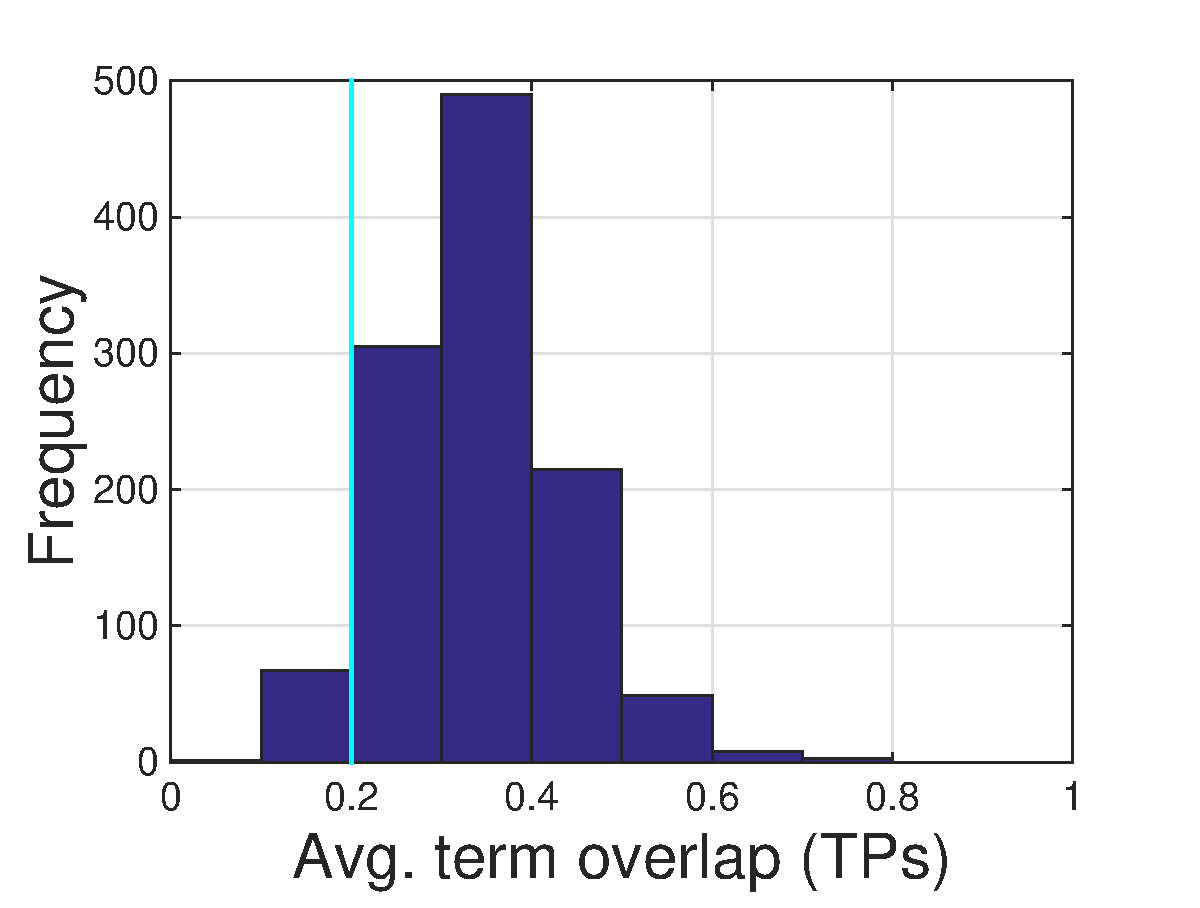
\includegraphics[width=5cm]{figs/to-tps.eps}}\subfigure[Query and FP patents.]{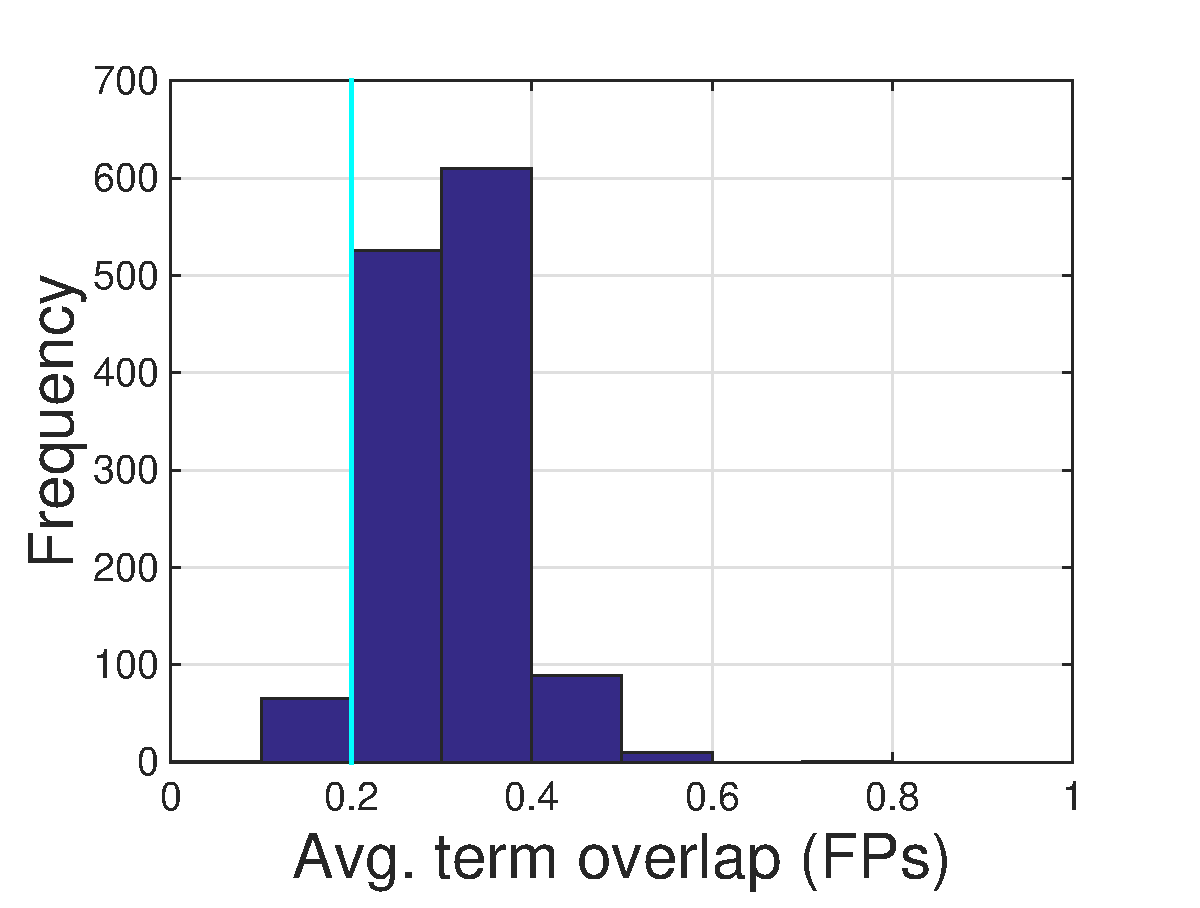
\includegraphics[width=5cm]{figs/to-fps.eps}}\subfigure[{Query and FN patents.}]{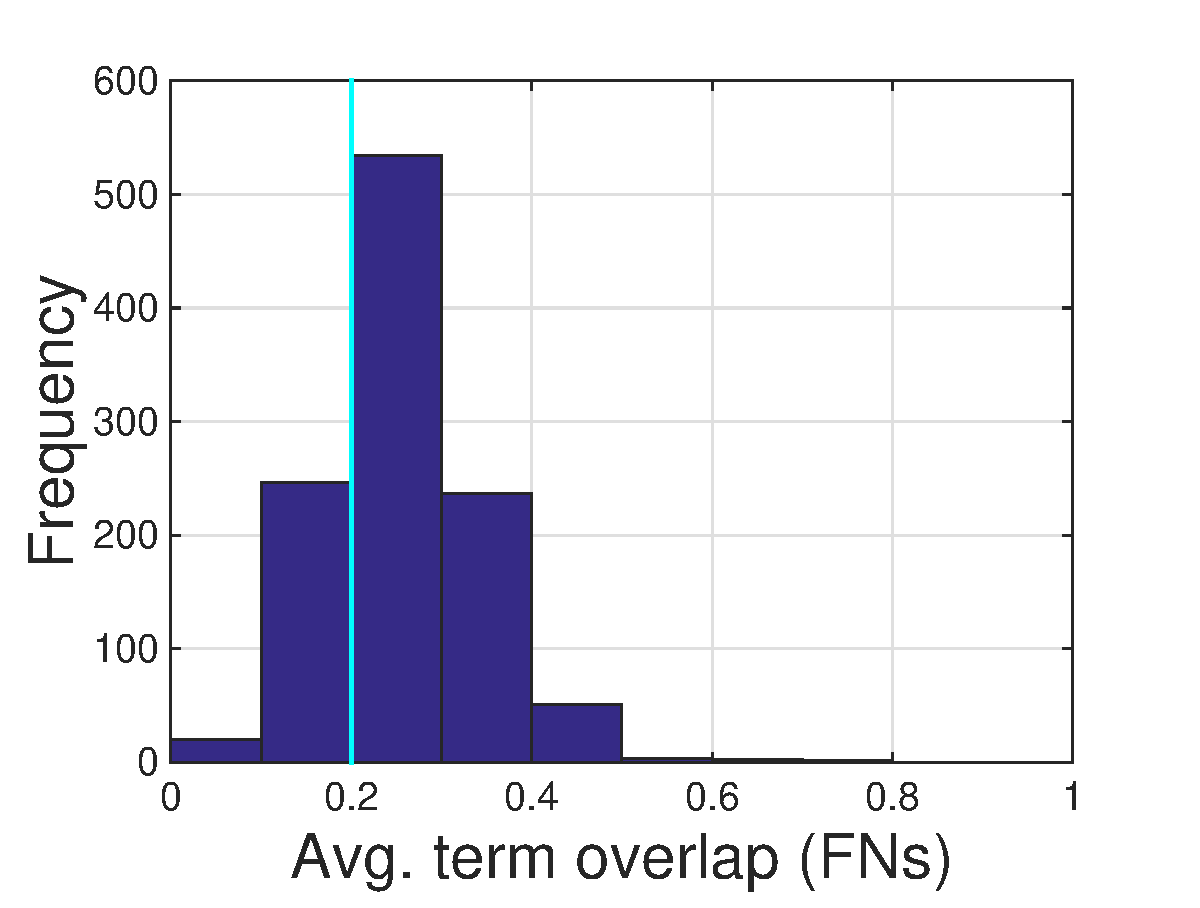
\includegraphics[width=5cm]{figs/to-fns.eps}}
\par\end{centering}

\protect\caption{The distribution of term overlap between the query and documents in three subsets (TP, FP, FN) over all queries in English test subset.}
\label{fig:overlap}
\end{figure}
%%%%%%%%%%%%%%%%%%%%%%%%%%%%%%%%%%%%%%%%%%%%%%%%%%%%%%%%%%%%%%
This experiment implicitly shows that a low or zero term match is not the main cause of low effectiveness in patent prior art search. In the next session, we explain a method to discriminate between the terms, which help the retrieval of relevant documents from those, which are not useful. 
%%%%%%%%%%%%%%%%%%%%%%%%%%%%%%%%%%%%%%%%%%%%%%%%%%%%%%%%%%%%%%
%%%%%%%%%%%%%%%%%%%%%%%%% SECTION 2 %%%%%%%%%%%%%%%%%%%%%%%%%%
%%%%%%%%%%%%%%%%%%%%%%%%%%%%%%%%%%%%%%%%%%%%%%%%%%%%%%%%%%%%%%
\section{Oracular Relevance Feedback System}
\label{sec:oraculrquery}
A query is optimal if it ranks all relevant documents before
those that are not relevant, it would lead to a ranking with an average precision of $1.0$. A query
is most likely to achieve a ranking that is as close to optimal as possible if it contains all terms that
appear in all relevant documents, but explicitly discounts all terms that occur in irrelevant documents~\citep{manning2008introduction}.

Inspired by the optimal query idea, we develop an oracular relevance feedback system, which
extracts terms from the judged relevant documents to derive an upper bound on performance of
standard Okapi BM25 and LM retrieval
algorithms for patent prior art search.
We, first, use the oracular relevance feedback to score query terms. 
Then, we run some experiments related to the existence of the useful terms inside the patent query.   
Finally, we analyse the system performance for two oracular query formulated by useful terms. 
%\subsection{Oracular Term Selection}
\subsection{Term Scoring}
\label{OracularTermSelection}
After an initial run of the patent query, we build a vocabulary set out of all terms appearing in top-100 retrieved documents; then we use judged relevant documents to score each term. 
We calculate an oracular relevance feedback score ($RF(t,Q)$) for each term $t$ in the top-100
retrieved documents given the query $Q$ as follows:
%%%%%%%%%%%%%%%%%%%%%%%%%%%%%%%%%%%%%%%%%%%%%%%%%%%%%%%%%%%%%%
\begin{equation}
RF(t,Q)=Rel(t)-Irr(t), 
 \label{eq:rfscore}
\end{equation}
\begin{displaymath}t\in \lbrace \mbox{terms in top-100 retrieved documents}\rbrace,\end{displaymath}
%%%%%%%%%%%%%%%%%%%%%%%%%%%%%%%%%%%%%%%%%%%%%%%%%%%%%%%%%%%%%%
where $ \mathit{Rel(t)} $ is the average term frequency in retrieved relevant patents, and $ \mathit{Irr(t)} $ is the average term frequency in retrieved irrelevant patents. According to the Equation \ref{eq:rfscore}, words appearing more frequently in relevant documents achieve higher RF score. We might assume that words, with a positive score, are \textit{useful terms} because they are more frequent in relevant patents while words, with a negative score, are \textit{noisy terms} because they appear more frequently in irrelevant patents. However in the following experiments, we empirically seek a threshold $\tau$ to pick useful terms. 

We yield the oracular relevance feedback score to: (i) find a pattern for the system performance versus useful terms; (ii) show the term overlap with useful terms and noisy terms for TP, FN patents; (iii)  examine the existence of useful terms in different sections of the patent query.
\subsection{Performance versus Useful Terms}
\label{PerformanceUsefulTerms}
%\paragraph{Performance versus Useful Terms}
%\ \\
We, intuitively, expect that queries, which contain more useful terms achieve higher performance. Hence in this experiment,
we investigate if more useful terms in the reference patent query leads to a higher performance. In other words, we seek for a pattern between the performance and the existence of the useful terms in initial patent query. 

We define four different criteria to select useful terms as follows:
\begin{enumerate}
\item terms with positive RF scores ($ RF(t, Q)>0) $);
\item terms with the score higher than the positive median score\\ ($ RF(t, Q)>RF(t_{+median}, Q) $);
\item terms with the score higher than a constant: 1, 5, and 10 ($ RF(t, Q)>1, 5, 10) $);
\item top-100 high-scored terms.
\end{enumerate}
For each query, we calculate the fraction of useful terms to all query terms. 
Figure~\ref{fig:overlap-r} shows the scatter plot of the recall versus this fraction. 
As it can be seen, unlike our first assumption, we do not see any correlation between the recall and the presence of useful terms in the query and the pattern for the recall is very noisy and irregular. 
We repeat the experiment for the average precision (AP). Figure~\ref{fig:overlap-p} shows the scatter plot of the AP versus the existence of useful terms in the query. Although it is slightly better than the recall and we can see a very weak correlation between AP and useful terms inside the query for top-scored words (e.g., $RF(t, Q)>10$), it does not demonstrate our first conjecture. 
This experiment also implicitly indicates that term mismatch between the patent query and relevant documents is 
not the main reason for the low effectiveness of the patent prior art search. 
%%%%%%%%%%%%%%%%%%%%%%%%%%%%%%%%%%%%%%%%%%%%%%%%%%%%%%%%%%%%%%
\begin{figure}[t!]
\begin{centering}
\subfigure[Useful terms: $ \{t|RF(t, Q)>0\} $]{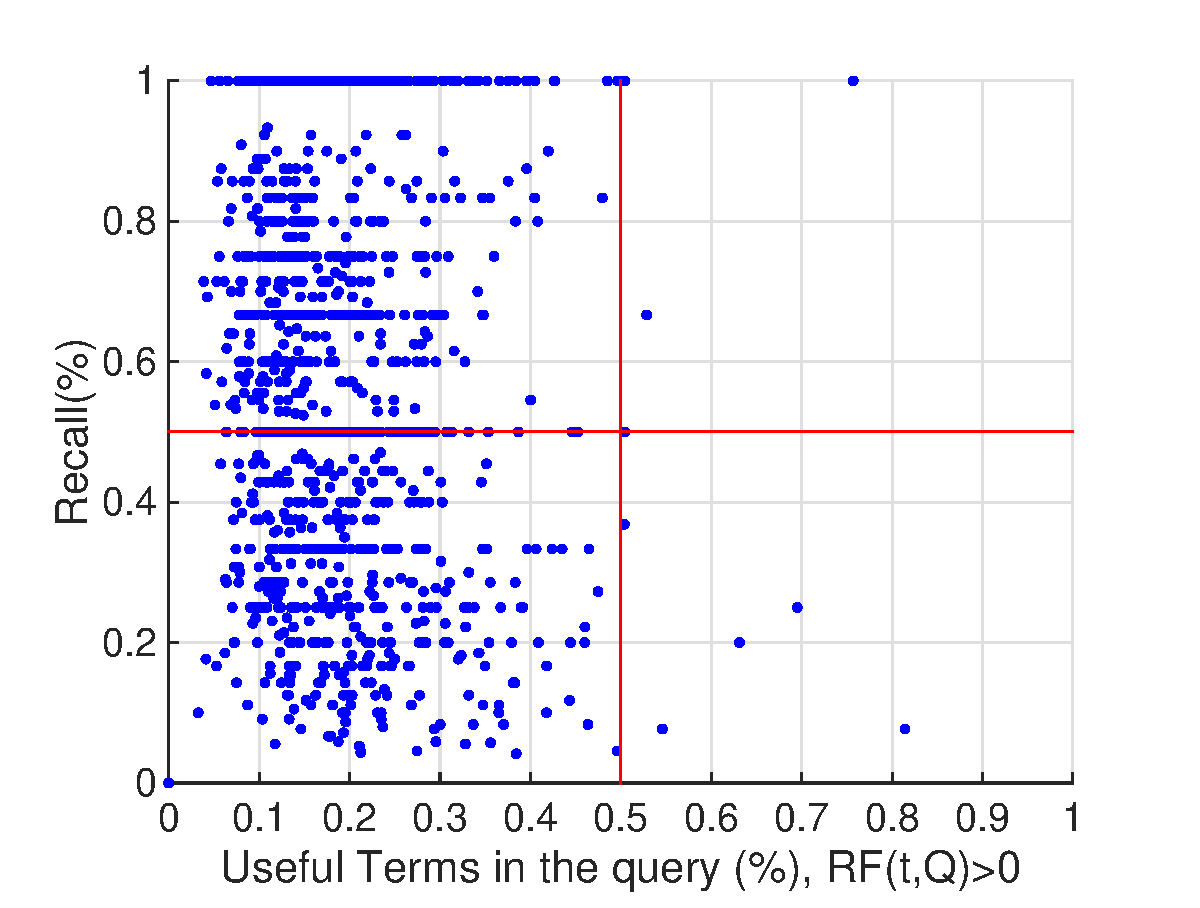
\includegraphics[width=6cm]{figs/greaterthan0-r.eps}} \hspace*{1.5cm} \subfigure[Useful terms: $ \{t|RF(t, Q)>RF(t_{+median})\} $]{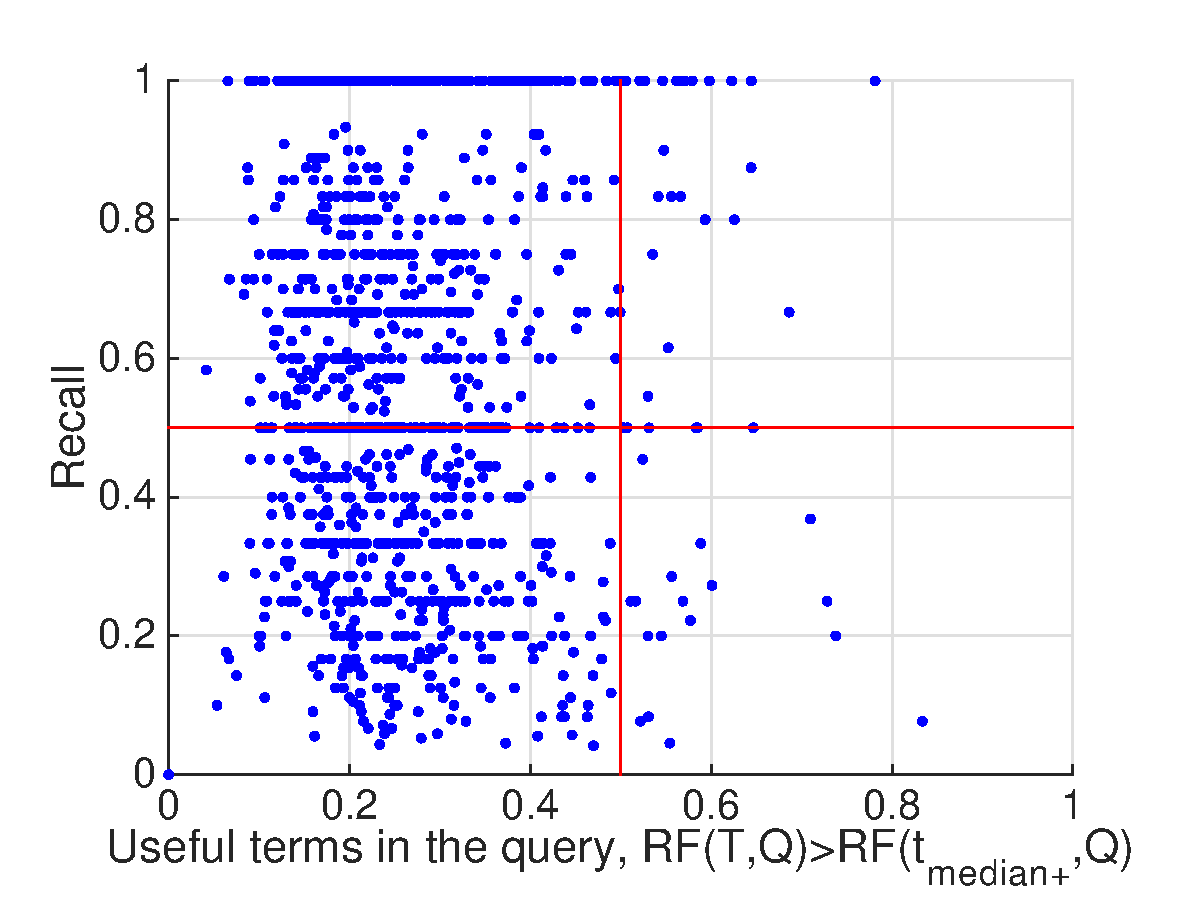
\includegraphics[width=6cm]{figs/greaterthanmedian-r.eps}}\\ \subfigure[{Useful terms: $ \{t|RF(t, Q)>1 \}$}]{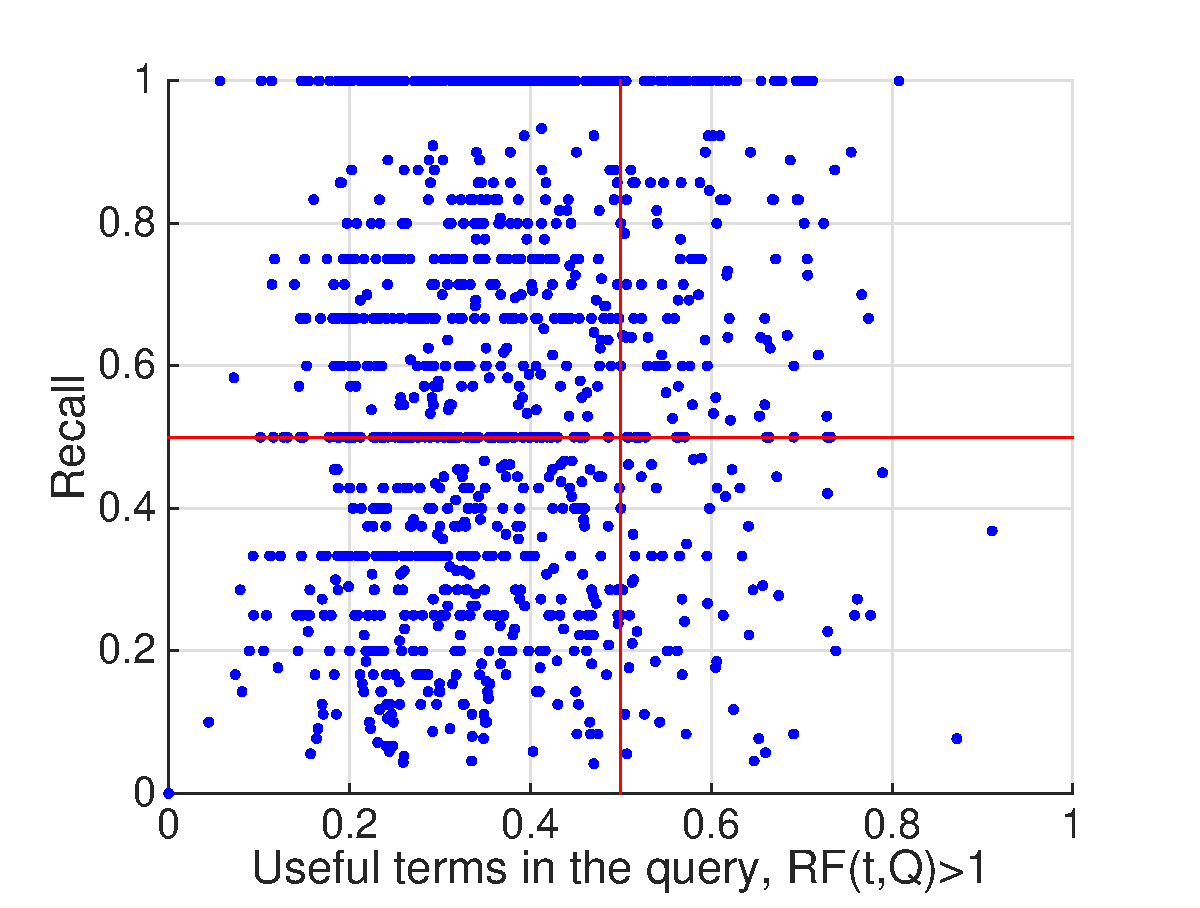
\includegraphics[width=6cm]{figs/greaterthan1-r.eps}} \hspace*{1.5cm} \subfigure[{Useful terms: top 100 high-scored terms}]{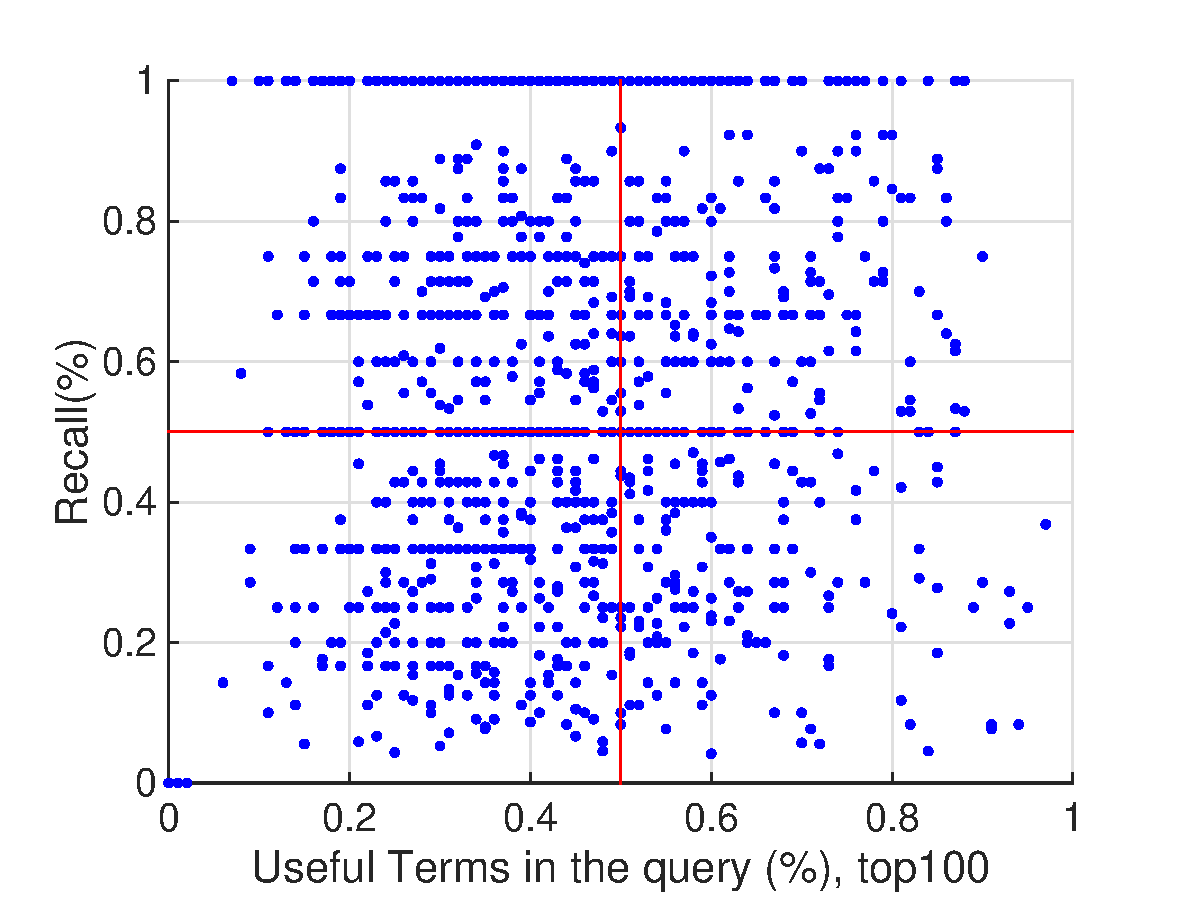
\includegraphics[width=6cm]{figs/top100-r.eps}}\\ \subfigure[{Useful terms: $ \{t|RF(t,Q)>5 \}$}]{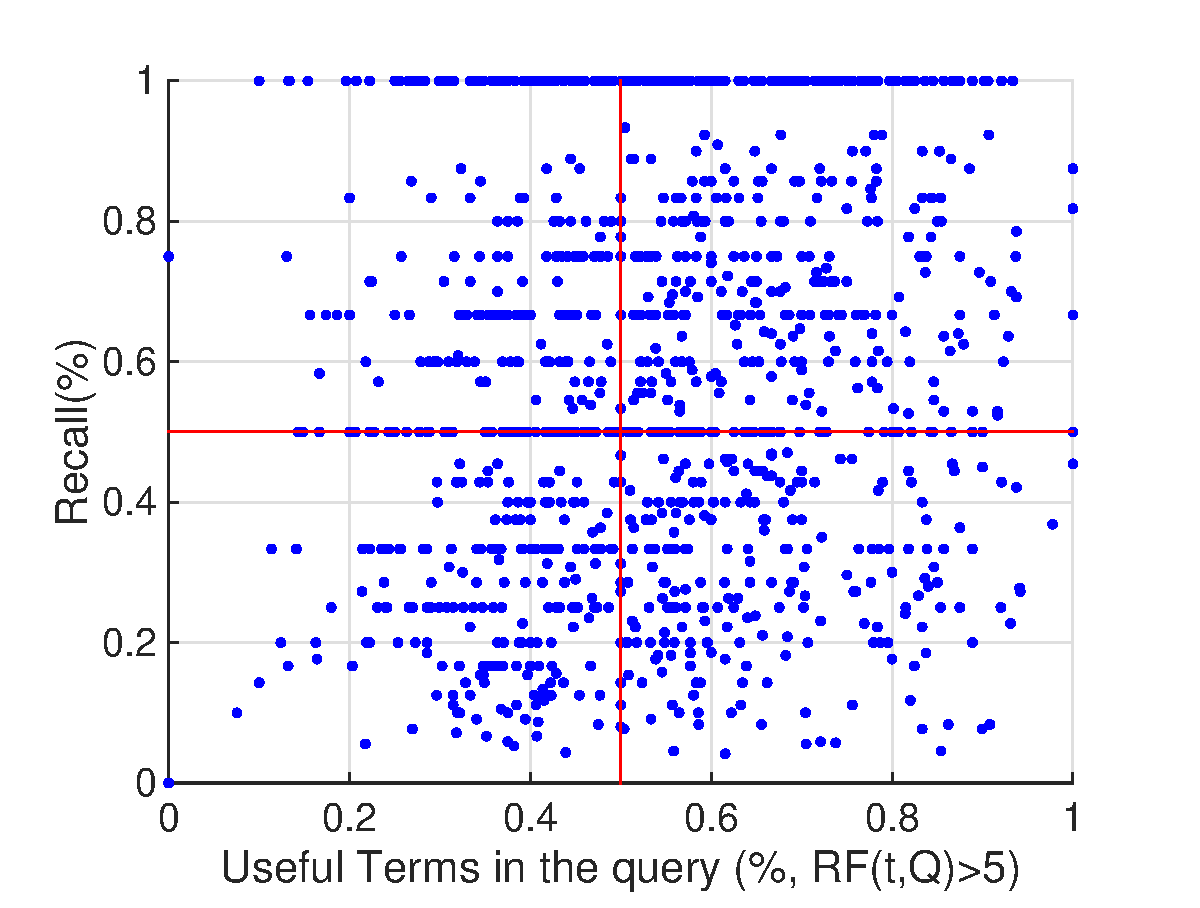
\includegraphics[width=6cm]{figs/greaterthan5-r.eps}} \hspace*{1.5cm} \subfigure[{Useful terms: $ \{t|RF(t, Q)>10\} $}]{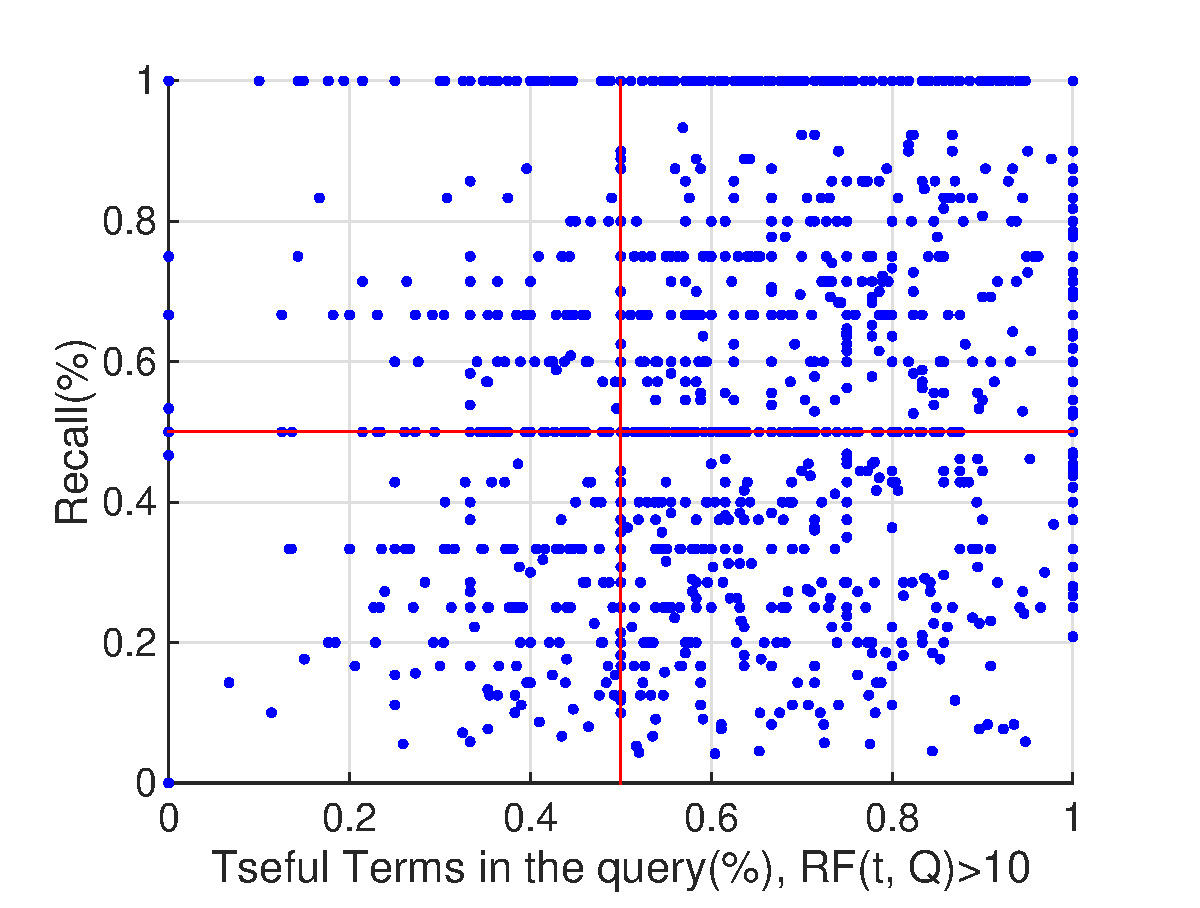
\includegraphics[width=6cm]{figs/greaterthan10-r.eps}}
\par\end{centering}

\protect\caption{Scatter plot of recall versus the existence of useful terms in query.}
\label{fig:overlap-r}
\end{figure}
%%%%%%%%%%%%%%%%%%%%%%%%%%%%%%%%%%%%%%%%%%%%%%%%%%%%%%%%%%%%%%
%%%%%%%%%%%%%%%%%%%%%%%%%%%%%%%%%%%%%%%%%%%%%%%%%%%%%%%%%%%%%%
\begin{figure}[t!]
\begin{centering}
\subfigure[Useful terms: $ \{t|RF(t, Q)>0\} $]{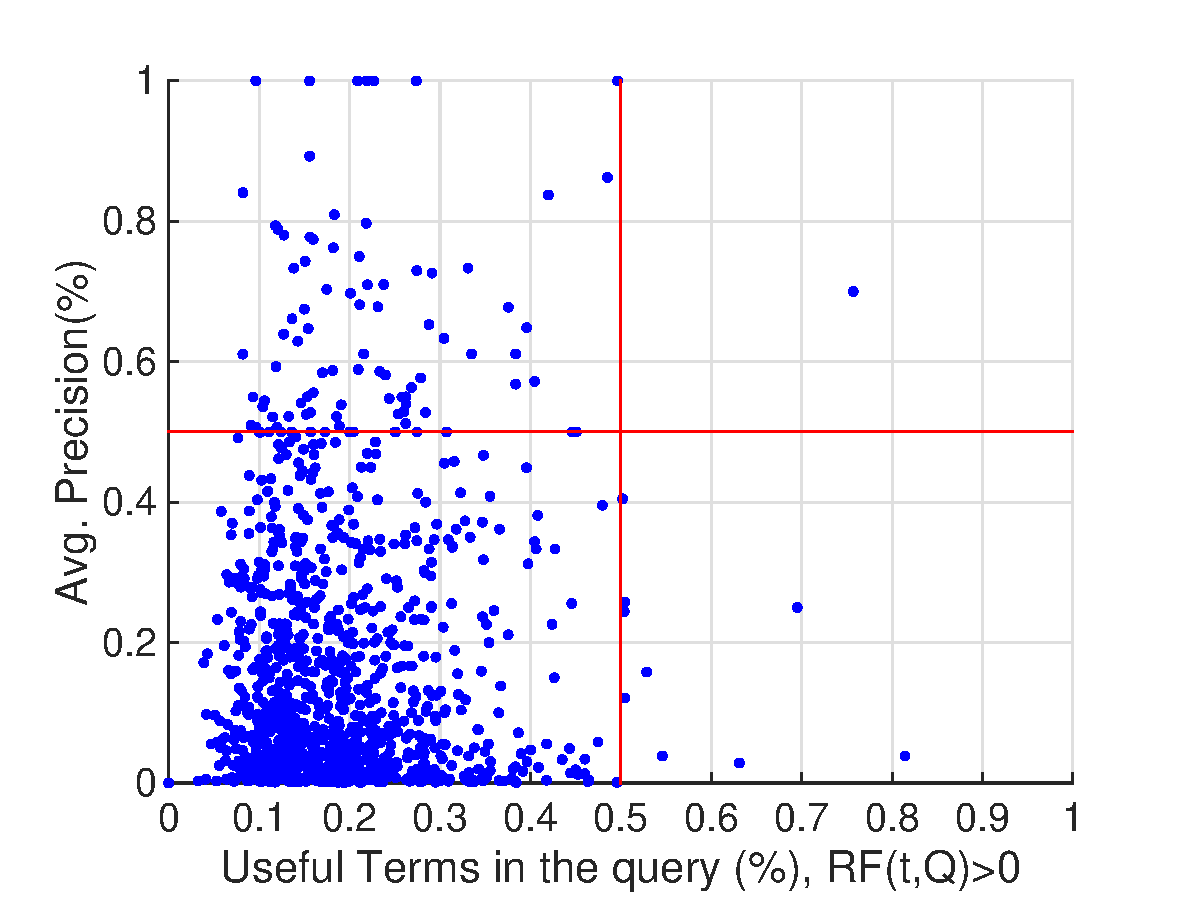
\includegraphics[width=6cm]{figs/greaterthan0-p}} \hspace*{1.5cm} \subfigure[Useful terms: $ \{t|RF(t, Q)>RF(t_{+median}, Q)\} $]{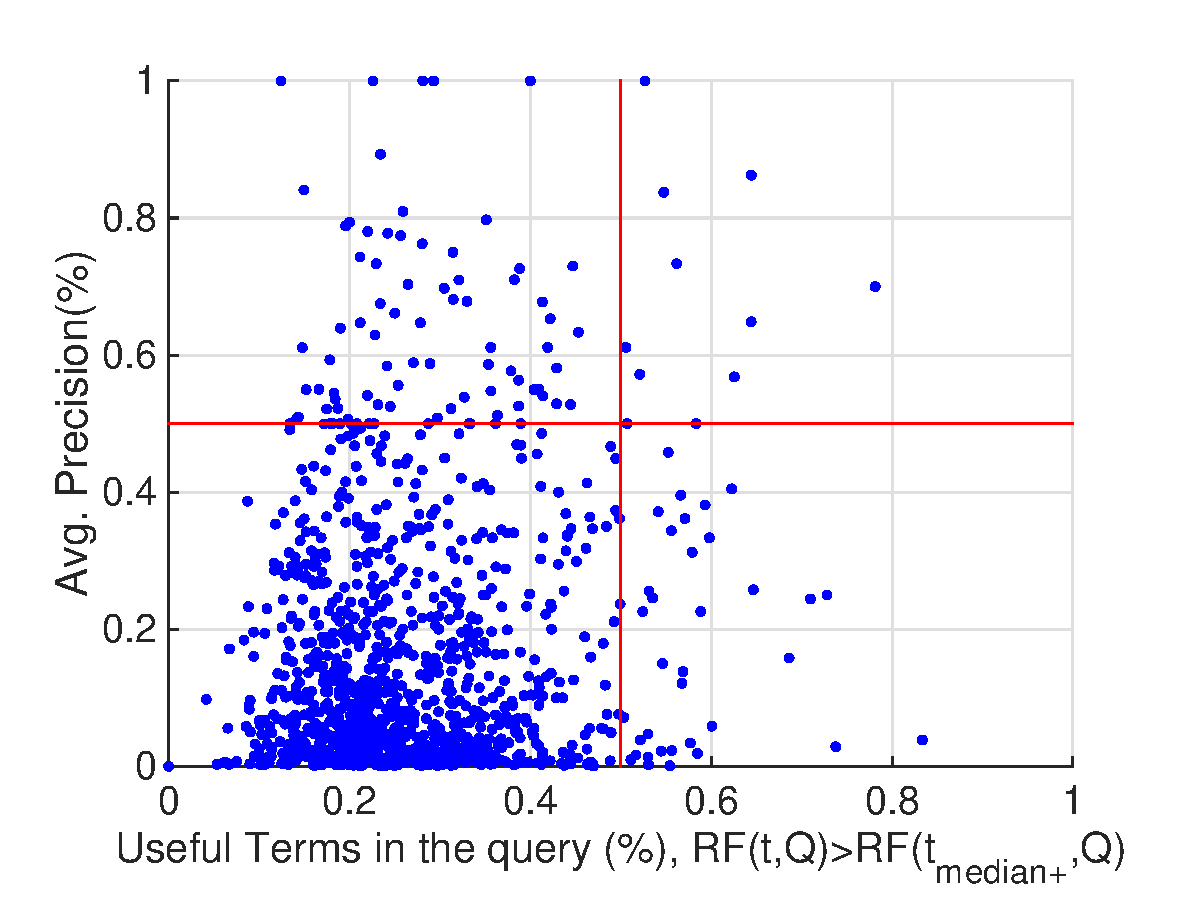
\includegraphics[width=6cm]{figs/greaterthammedian-p.eps}} \\%[-2ex]% 
\subfigure[{Useful terms: $ \{t|RF(t, Q)>1 \}$}]{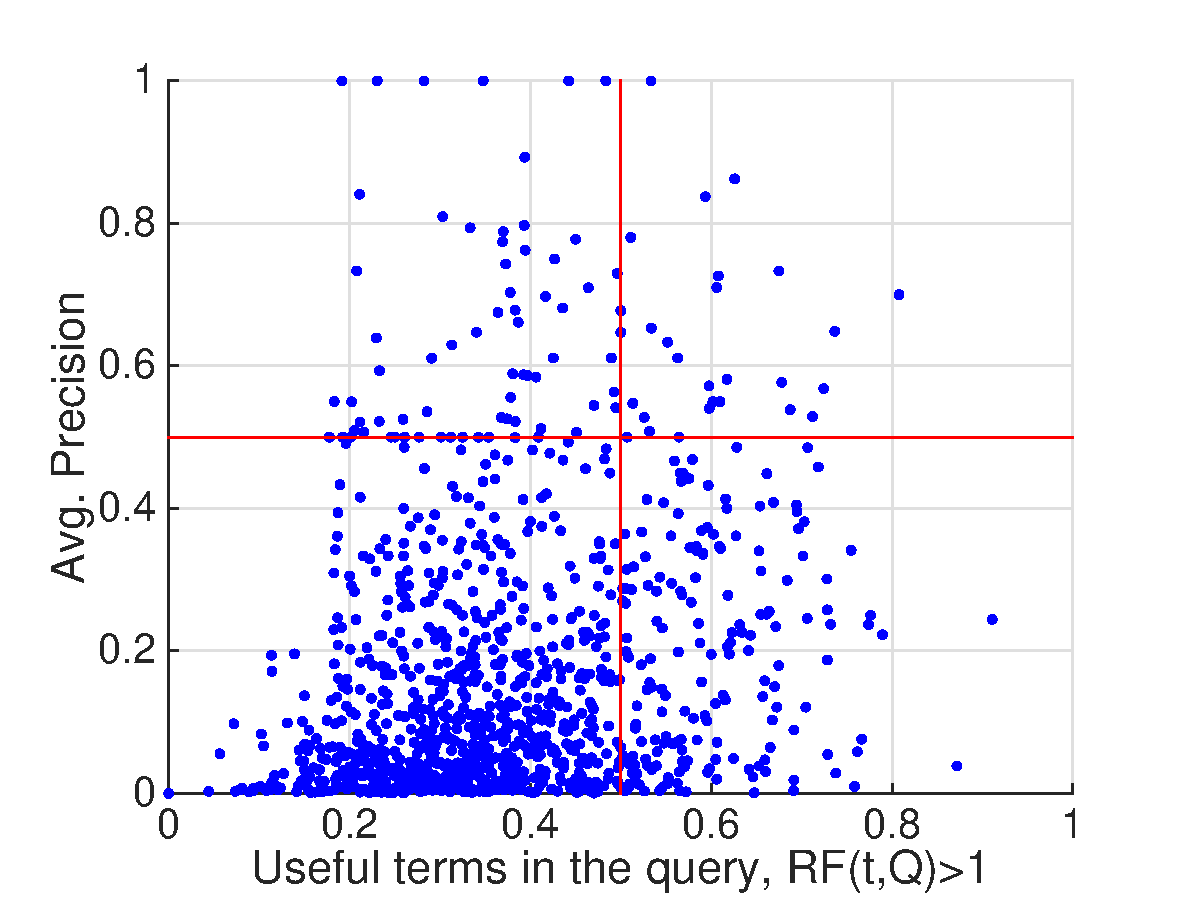
\includegraphics[width=6cm]{figs/greaterthan1-p.eps}} \hspace*{1.5cm} \subfigure[{Useful terms: top 100 high-scored terms}]{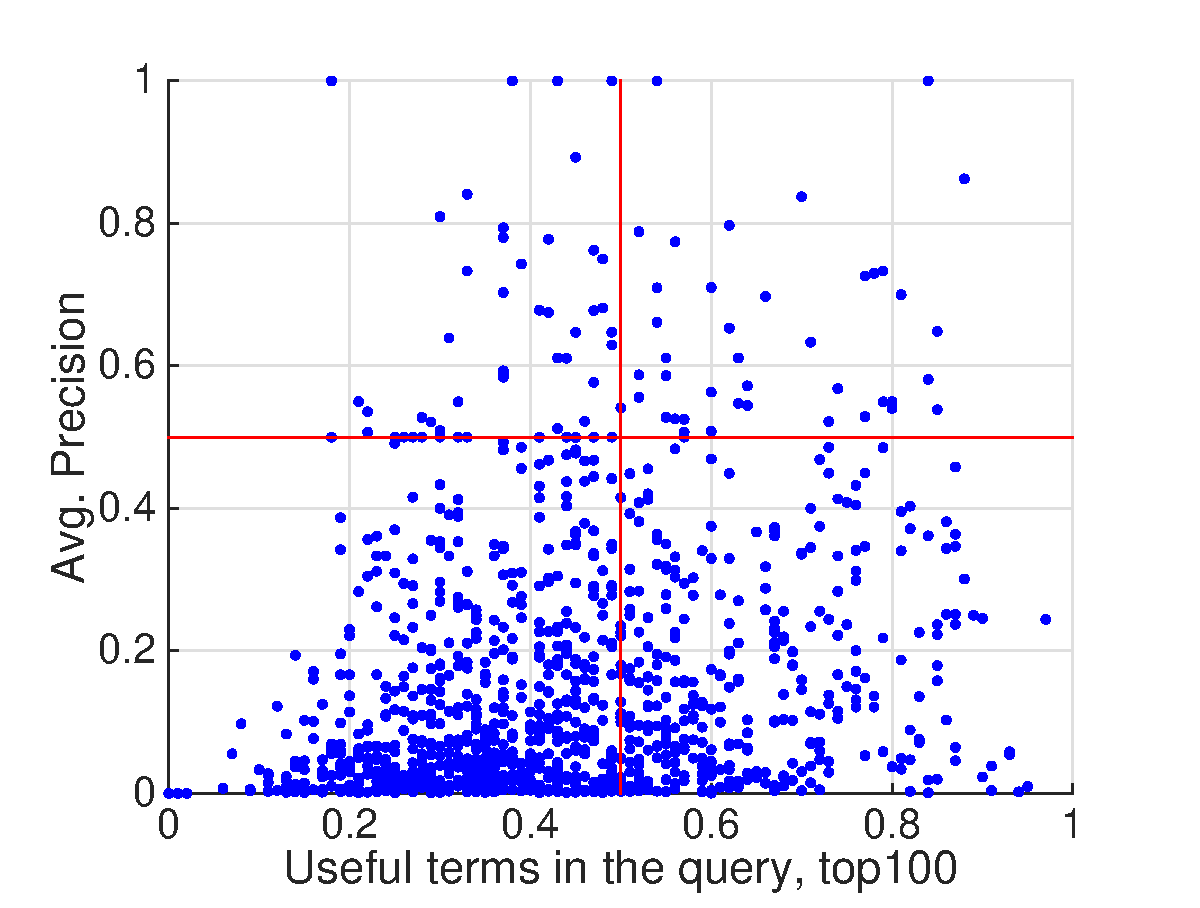
\includegraphics[width=6cm]{figs/top100-p.eps}}\\ %[-2ex]%
\subfigure[{Useful terms: $ \{t|RF(t,Q)>5 \}$}]{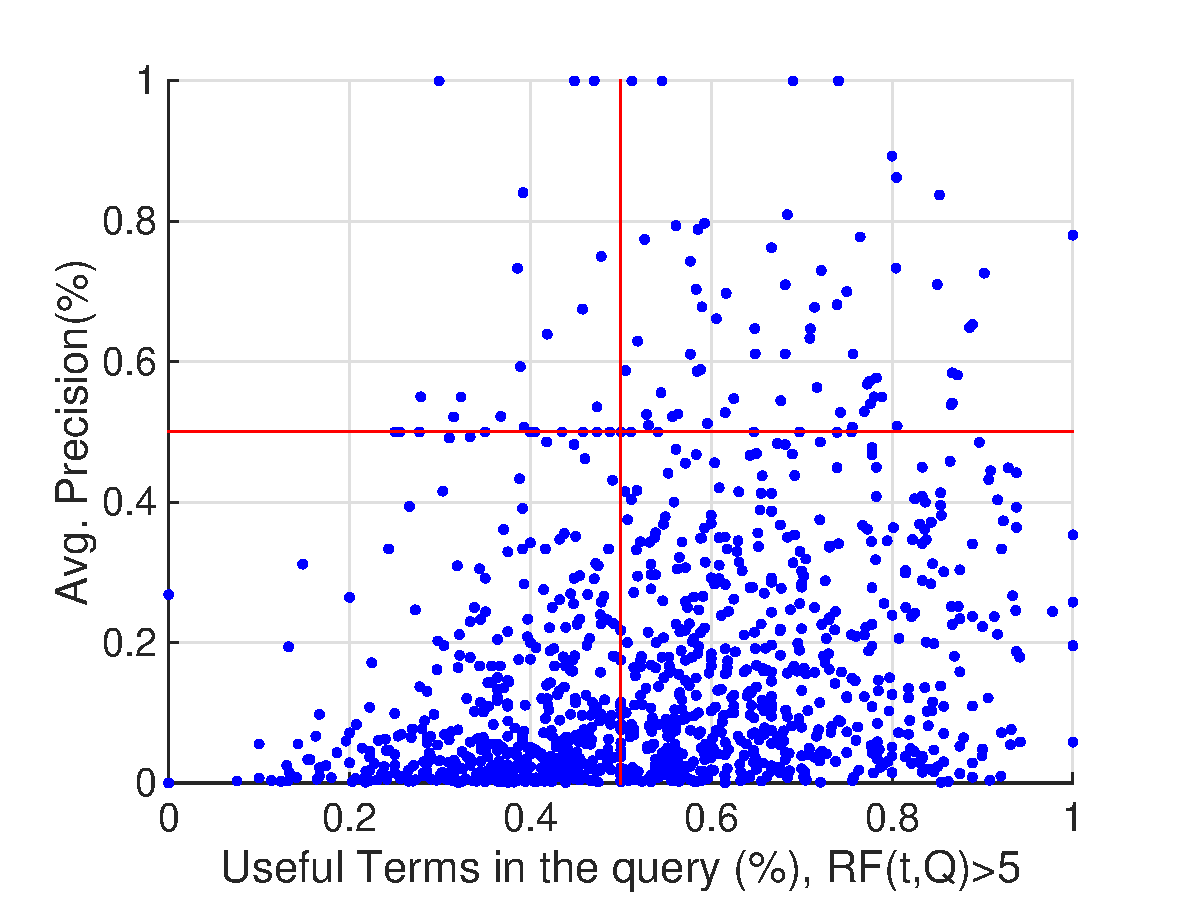
\includegraphics[width=6cm]{figs/greaterthan5-p.eps}} \hspace*{1.5cm} \subfigure[{Useful terms: $ \{t|RF(t, Q)>10\} $}]{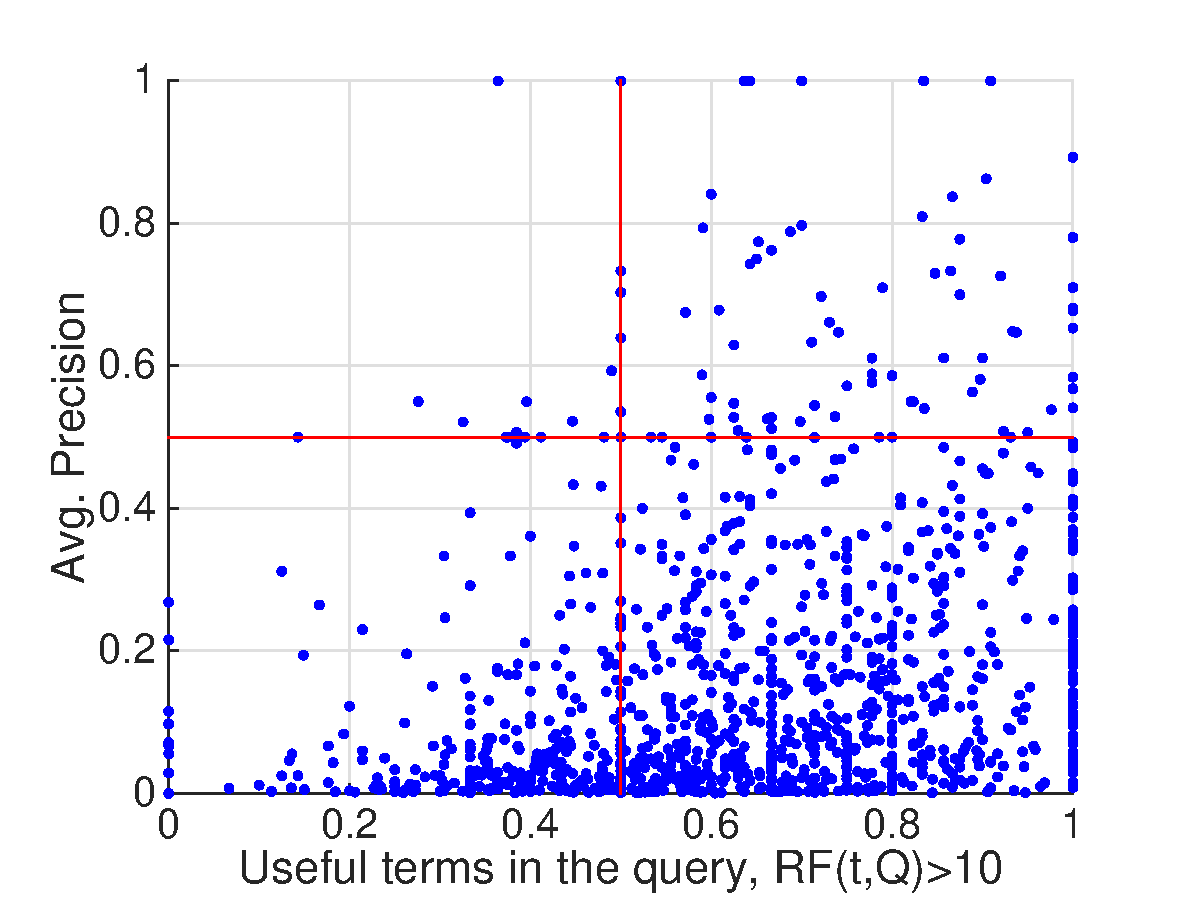
\includegraphics[width=6cm]{figs/greaterthan10-p.eps}}
\par\end{centering}

\protect\caption{Scatter plot of average precision (AP) versus the existence of useful terms in query.}
\label{fig:overlap-p}
\end{figure}
%%%%%%%%%%%%%%%%%%%%%%%%%%%%%%%%%%%%%%%%%%%%%%%%%%%%%%%%%%%%%%
\subsection{Term Overlap with Useful Terms and Noisy Terms}
%\paragraph{Term Overlap with Useful Terms and Noisy Terms}
%\ \\
In the second experiment, we check the term overlap with useful terms and noisy terms for TP and FP patents. Figure \ref{fig:usefulnoisy} shows that relevant patents have a higher term overlap with the useful terms while irrelevant patents have a higher term overlap with the noisy terms. This experiment shows that noisy terms cause the system to retrieve irrelevant patents at top of the list. 
%%%%%%%%%%%%%%%%%%%%%%%%%%%%%%%%%%%%%%%%%%%%%%%%%%%%%%%%%%%%%%
\begin{figure}[t!]
%[htpb]
\begin{centering}
\subfigure[TPs]{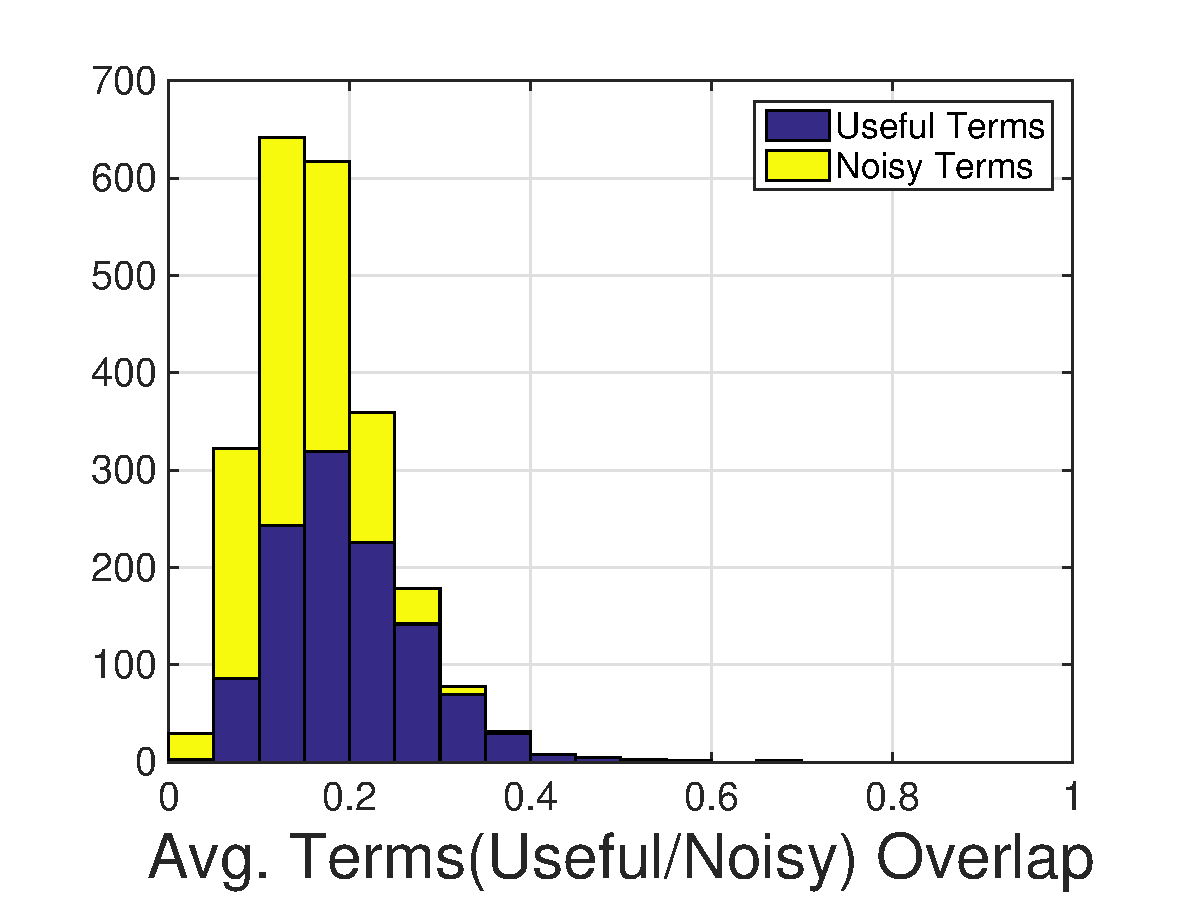
\includegraphics[width=6cm]{figs/stackedTPs.eps}} \hspace*{1.5cm} \subfigure[FPs]{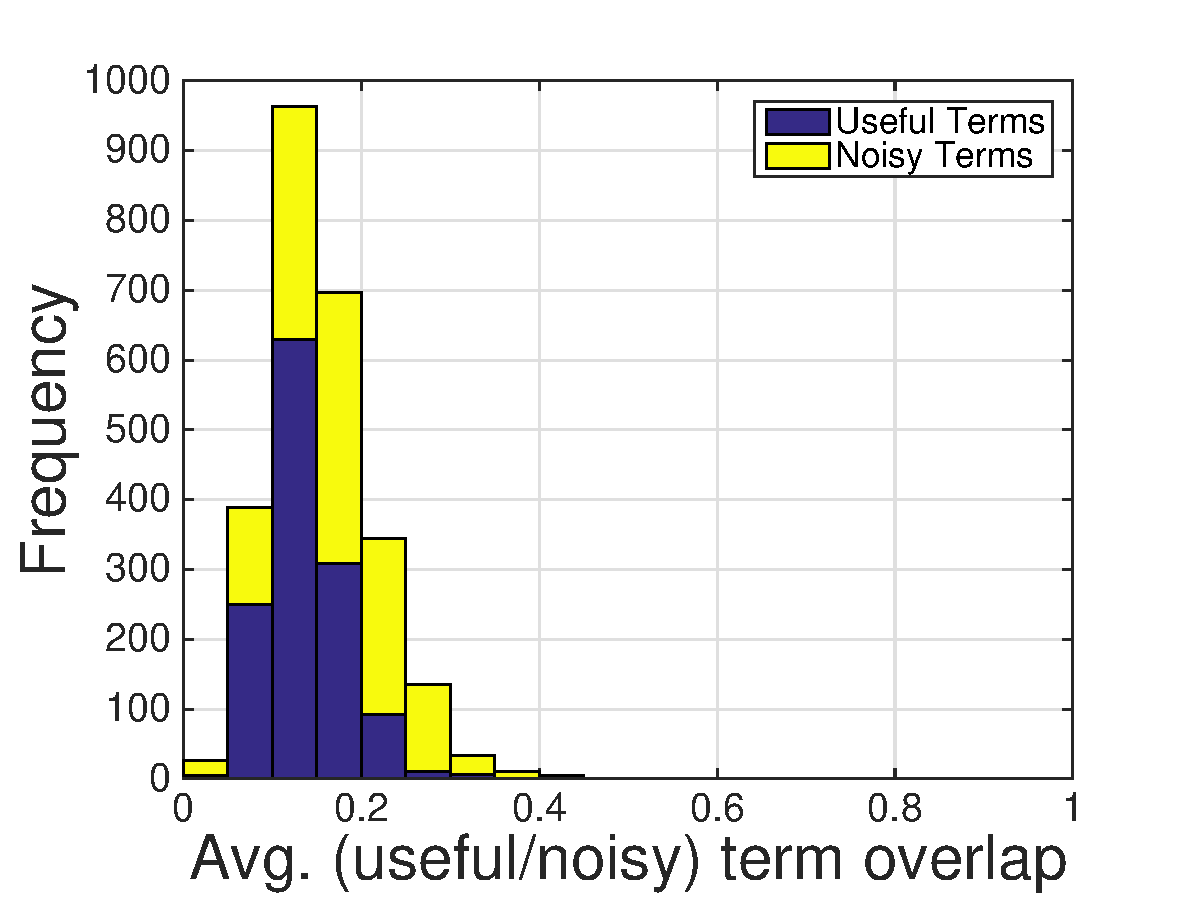
\includegraphics[width=6cm]{figs/stackedFPs.eps}} 
\par\end{centering} 

\protect\caption{The distribution of the term overlap between the query and useful terms/noisy terms in TPs and FPs. Relevant patents have higher term overlap with useful terms while irrelevant patents have higher term overlap with noisy terms.}
\label{fig:usefulnoisy}
\end{figure}
%%%%%%%%%%%%%%%%%%%%%%%%%%%%%%%%%%%%%%%%%%%%%%%%%%%%%%%%%%%%%%
%We hypothesized that a query, formulated by only the \textit{ useful terms}, is the best possible query we can make since they are all frequent in relevant patents but rare in irrelevant ones. 
\subsection{Useful Terms in Different Sections of Patents}
%\paragraph{Useful Terms in Different Sections of Patents}
%\ \\
%%%%%%%%%%%%%%%%%%%%%%%%%%%%%%%%%%%%%%%%%%%%%%%%%%%%%%%%%%%%%%
\begin{table*}[t!]
  \begin{center}
   \caption{Average number of useful terms in the different sections of patent query}
  \input table/usefultermsinsections.tex   
  \label{tab:usefultermsinsections}
  \end{center}  
\end{table*}
%\FloatBarrier
%%%%%%%%%%%%%%%%%%%%%%%%%%%%%%%%%%%%%%%%%%%%%%%%%%%%%%%%%%%%%%
%%%%%%%%%%%%%%%%%%%%%%%%%%%%%%%%%%%%%%%%%%%%%%%%%%%%%%%%%%%%%%
\begin{table*}[t!]
  \begin{center}
   \caption{Average percentage of useful terms in the different sections of patent query}
  \input table/usefultermsinsections-p.tex   
  \label{tab:usefultermsinsections-p}
  \end{center}  
\end{table*}
%%%%%%%%%%%%%%%%%%%%%%%%%%%%%%%%%%%%%%%%%%%%%%%%%%%%%%%%%%%%%%
Patents are structured documents containing title, abstract, description, and claims (Section~\ref{StructureofPatents}). In this experiment, we investigate the existence of useful terms in different sections of patents. 
Table \ref{tab:usefultermsinsections} shows the average number of useful terms in different sections of a patent query.  
As it can be seen, description has the highest number of useful terms in both cases where RF score threshold $ \tau $ is $0$ and $1$. When $ \tau = 0 $, the average number of the useful terms in description is quite twice of when $ \tau = 1 $. Compared to other sections, description contains more useful terms, which proves why we achieved higher performance querying with description (Section~\ref{sec:settings}).
Table \ref{tab:usefultermsinsections-p} shows the average percentage of useful terms in different sections of a patent query. It shows that, overall, useful terms constitute less than 50\% of the whole words in each section of patent queries. For example, only 27\% of the description of a patent query are useful terms on average and the rest are irrelevant terms. 
%\subsubsection{Useful Terms in Different Sections}
\subsection{Oracular Query Formulation}
\label{sec:OracularQueryFormulation}
As we illustrated in Section~\ref{PerformanceUsefulTerms}, we could not find an informative pattern for the performance and the existence of the useful terms in patent query.
In this section, we examine the system effectiveness for queries formulated using terms selected by oracular relevance feedback system.
We formulate two different oracular queries.

The \textit{first} query is formulated by selecting terms in the top-100 retrieved documents using oracular relevance feedback score and we call it oracular query:
%%%%%%%%%%%%%%%%%%%%%%%%%%%%%%%%%%%%%%%%%%%%%%%%%%%%%%%%%%%%%%
\begin{equation}
Oracular \; Query = \{t \in top-100|RF(t, Q)>\tau\}.   
 \label{eq:oq}
\end{equation}
%%%%%%%%%%%%%%%%%%%%%%%%%%%%%%%%%%%%%%%%%%%%%%%%%%%%%%%%%%%%%% 
%%%%%%%%%%%%%%%%%%%%%%%%%%%%%%%%%%%%%%%%%%%%%%%%%%%%%%%%%%%%%%
\begin{figure}[t!]
\begin{centering}
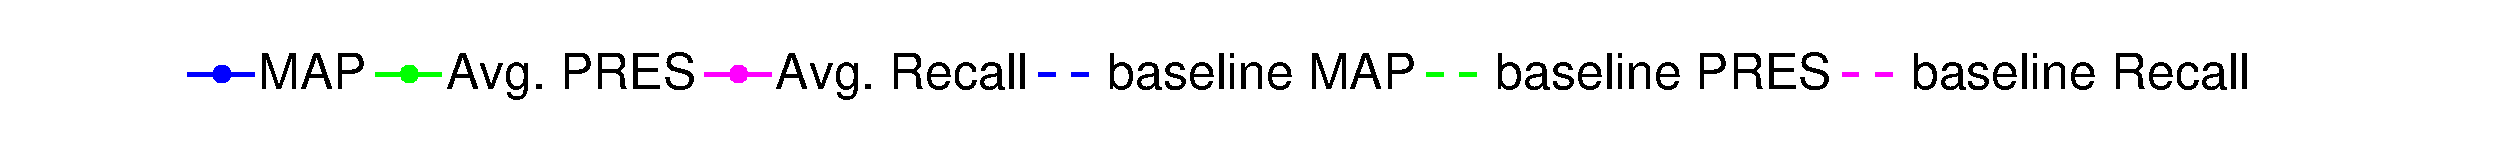
\includegraphics[width=15cm]{figs/lo}
\par\end{centering}

\begin{centering}
\subfigure[Oracular query performance versus the threshold $\tau$.\label{fig:oracular-a}]{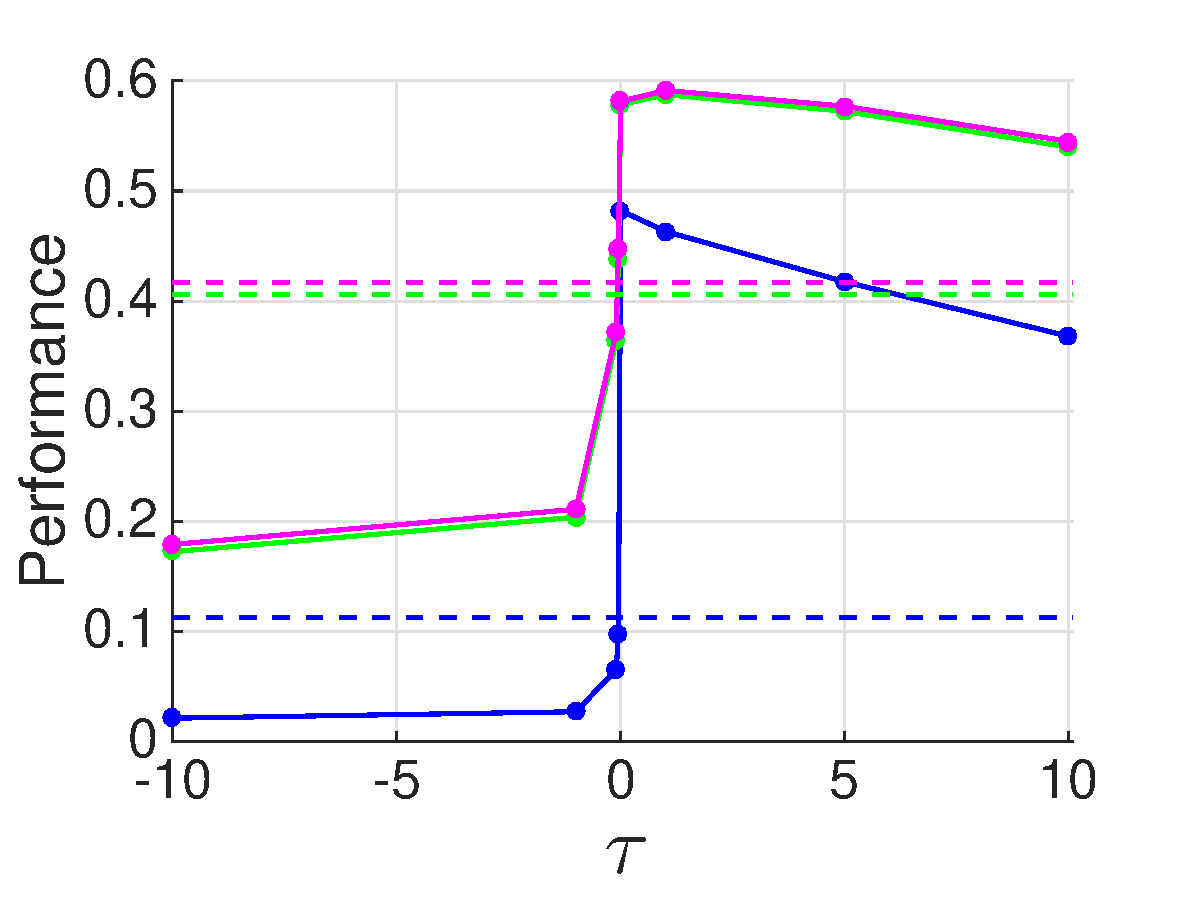
\includegraphics[width=6cm]{figs/oracularq.eps}} \hspace*{.5cm} \subfigure[Oracular query performance versus the query size.\label{fig:oracular-b}]{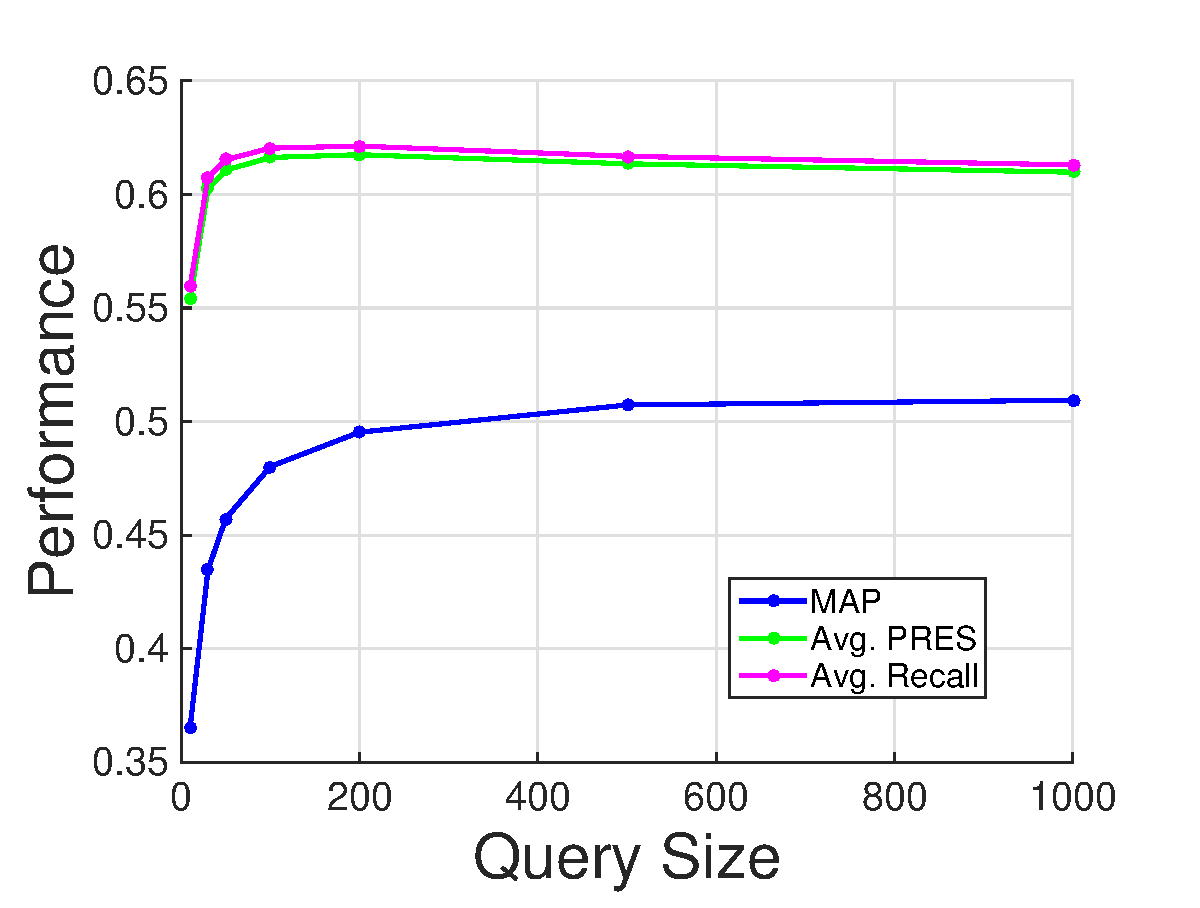
\includegraphics[width=6cm]{figs/oracularq-size.eps}} 
\par\end{centering} 
\protect\caption{Oracular query performance versus various values of the threshold $\tau$ and query size}
\label{fig:oracular}
\end{figure}
%%%%%%%%%%%%%%%%%%%%%%%%%%%%%%%%%%%%%%%%%%%%%%%%%%%%%%%%%%%%%%
First, we empirically seek to evaluate the threshold $\tau$ on $RF(t,Q)$ yielding the best oracular query.
Figure \ref{fig:oracular-a} shows that the performance changes by the values of $\tau$ and peaks at $\tau=0$. We also remark that the performance jumps notably over the baseline for the oracular query formulated by the Equation \ref{eq:oq}. Second, we seek for the best number of terms to formulate the oracular query. 
Figure~\ref{fig:oracular-b} shows that the performance increases notably when we include terms up to 200 while formulating a query, however it remains quit unchanged when we include more than 200 terms. 
%Next, inspired by Maxwell and Croft's work~\citep{maxwell2013compact} that emphasise on the importance of query words, 

We seek to establish that the terms within a reference patent query are sufficient for a strong performance, so, we formulate the \textit{second} query by selecting oracular terms that also occur in the reference patent query. We call it oracular patent query:
%%%%%%%%%%%%%%%%%%%%%%%%%%%%%%%%%%%%%%%%%%%%%%%%%%%%%%%%%%%%%%
\begin{equation}
 Oracular \; Patent \; Query = \{t\in Q|RF(t, Q)>\tau\}.   
 \label{eq:score}
\end{equation}
%%%%%%%%%%%%%%%%%%%%%%%%%%%%%%%%%%%%%%%%%%%%%%%%%%%%%%%%%%%%%%
%%%%%%%%%%%%%%%%%%%%%%%%%%%%%%%%%%%%%%%%%%%%%%%%%%%%%%%%%%%%%%
\begin{figure}[t!]
\begin{centering}
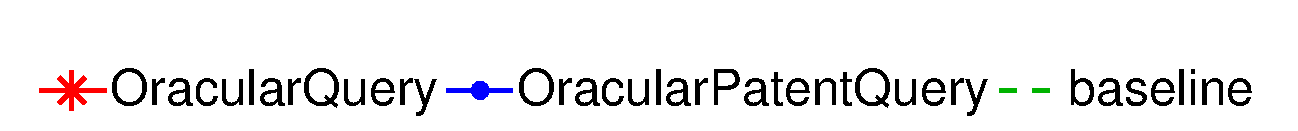
\includegraphics[width=9cm]{figs/l1}
\par\end{centering}

\begin{centering}
\subfigure[Mean Average Precision $\tau$.\label{fig:oracularpq-a}]{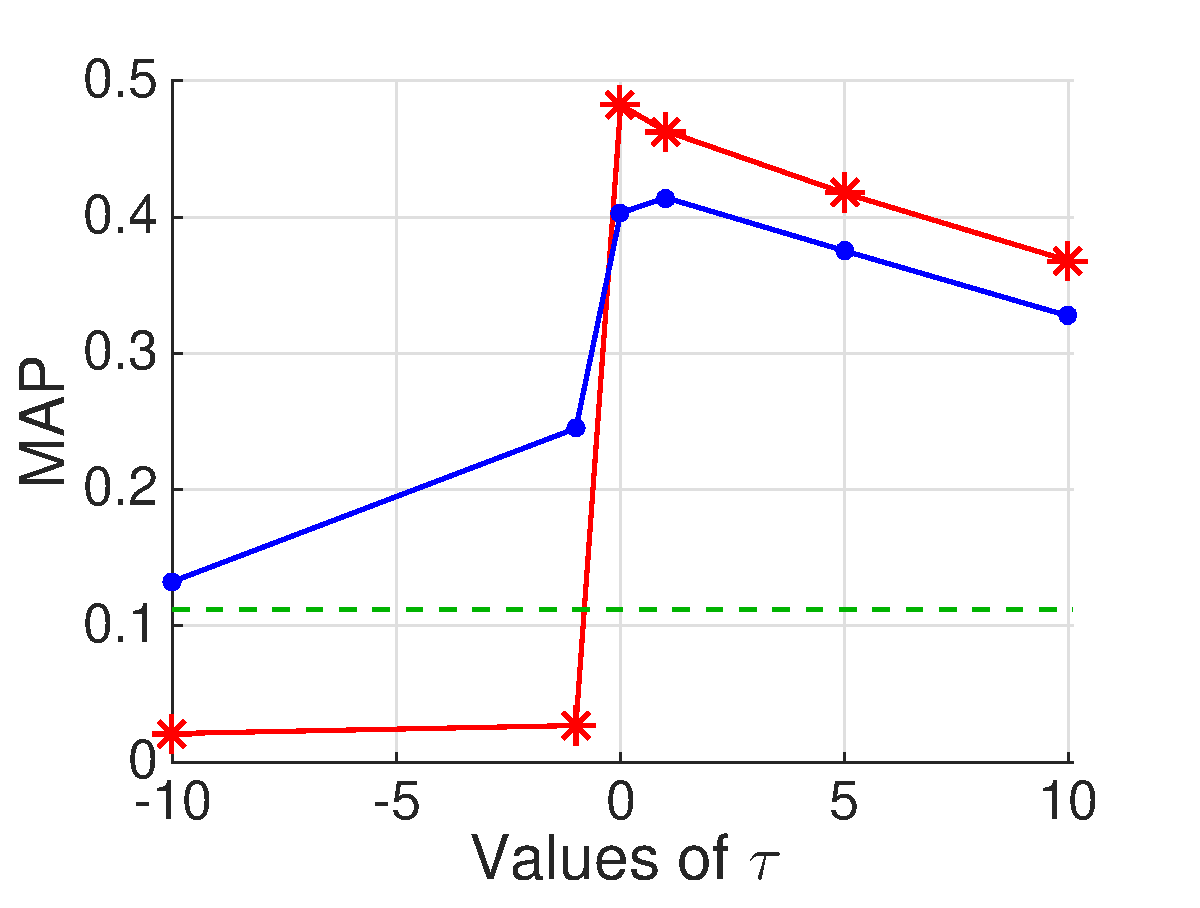
\includegraphics[width=6cm]{figs/fig1_map.eps}} 
\hspace*{1.5cm} \subfigure[Average Recall\label{fig:oracularpq-b}]{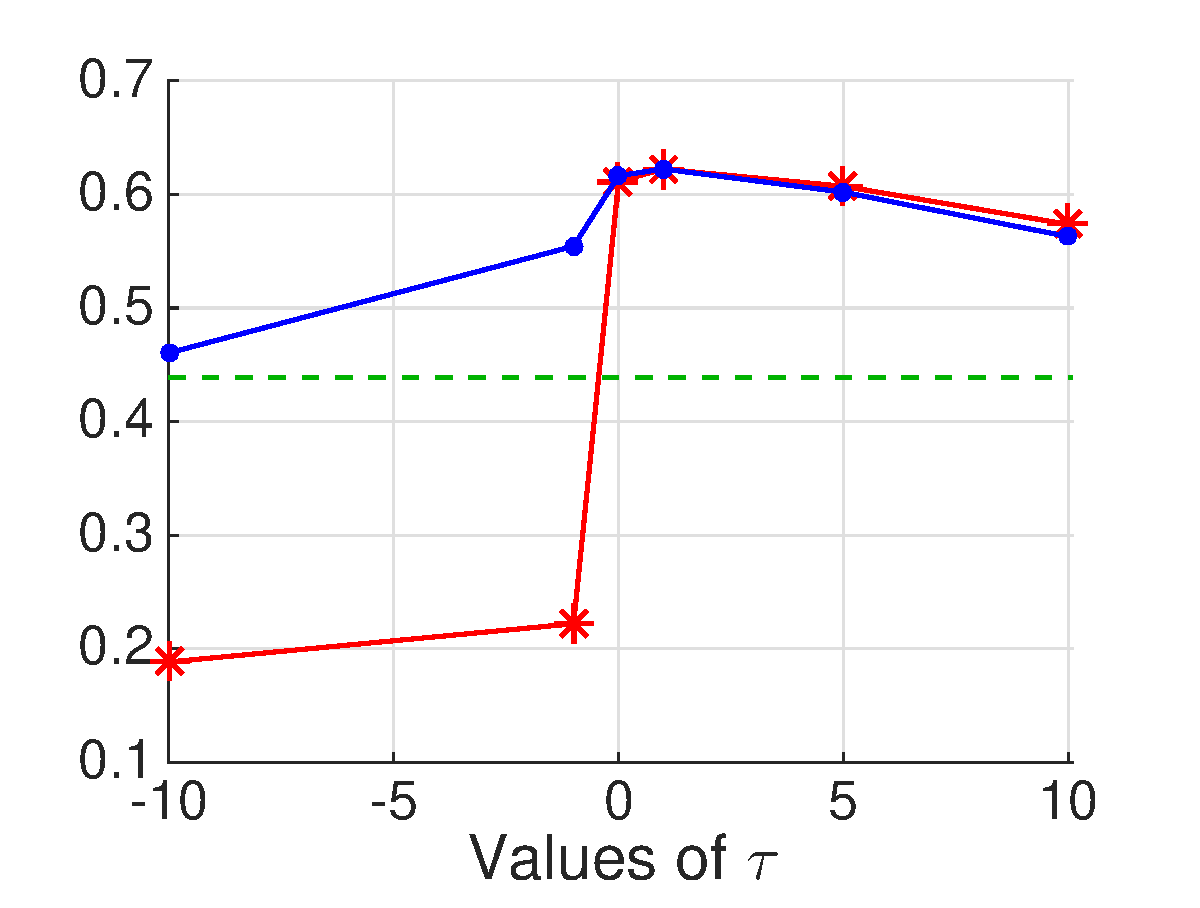
\includegraphics[width=6cm]{figs/fig1_recall.eps}} 
\par\end{centering} 

\protect\caption{Comparing the performance of oracular query and oracular patent query for various values of the threshold $\tau$}
\label{fig:oracularpq}
\end{figure}
%\begin{figure}[t!]
%   \centering
%   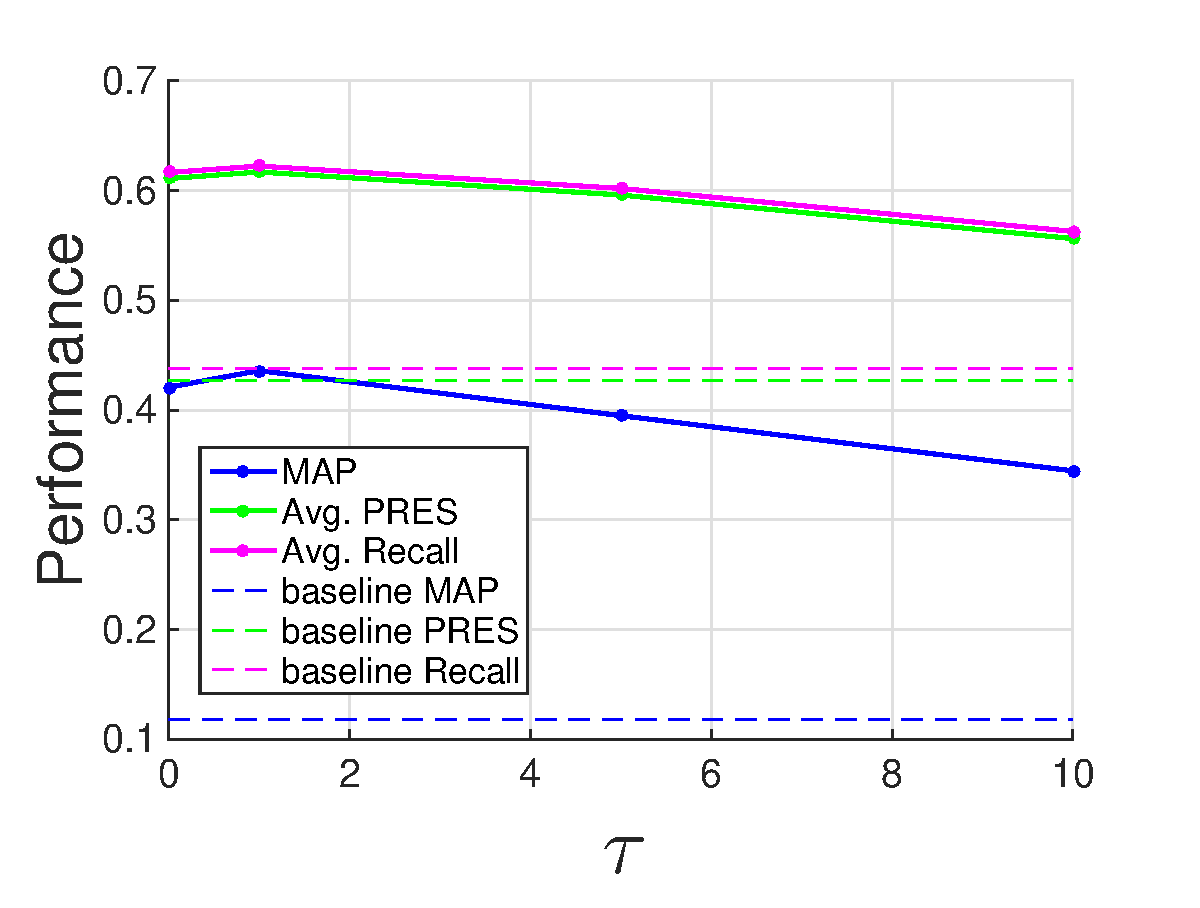
\includegraphics[width=0.50\textwidth,height=55mm]{figs/oracularpq.eps}
%   \caption{oracular patent query performance versus the threshold $\tau$.}   
%   \label{fig:oracularpq} 
%\end{figure}
%%%%%%%%%%%%%%%%%%%%%%%%%%%%%%%%%%%%%%%%%%%%%%%%%%%%%%%%%%%%%%
%%%%%%%%%%%%%%%%%%%%%%%%%%%%%%%%%%%%%%%%%%%%%%%%%%%%%%%%%%%%%%
\begin{table}[t!]
  \begin{center}
  \scriptsize
   \caption{Performance for the patent query (PQ/baseline), two variants of the oracular query (OracularQ, OracularPQ), and top CLEF-IP 2010 competitor (PATATRAS).}
   \vspace*{1ex}
  \input table/optquery.tex   
  \label{tab:optquery}
  \end{center}  
\end{table}
%%%%%%%%%%%%%%%%%%%%%%%%%%%%%%%%%%%%%%%%%%%%%%%%%%%%%%%%%%%%%%
\vspace*{-1cm}
\paragraph{Baseline versus Oracular Query}
\ \\
First, we investigate the ideal threshold setting $\tau$ for the
oracular queries as shown in Figure \ref{fig:oracularpq}.  Notably,
there is a rather unexpected steep dropoff in performance for both
oracular queries when slightly noisy terms are included
(i.e., $\tau$ just slightly less than 0).  However, this dropoff is
less pronounced for the
oracular patent query indicating that restriction to query terms in the
reference patent may reduce the impact of the noisy terms that are present.
While the oracular query and oracular patent query peak
at slightly different thresholds ($\tau = 0$ and $\tau = 1$, respectively), 
either value of $\tau$ yields good performance.
However, values of $\tau > 1$
demonstrate a stronger relative decrease in performance due to the exclusion 
of a large number of useful terms.

In Table~\ref{tab:optquery}, we compare our best oracular relevance
queries with both the baseline patent query and the PATATRAS
system.  In general we found BM25 and LM to offer very similar
performance.  Our subsequent results use only LM due to space
limitations although results for BM25 are very similar.  More
importantly, the oracular query using $\tau=0$ far
outperforms the baseline and approximately performs twice as well on
MAP as the PATATRAS system, the best competitor in CLEF-IP 2010.  The
MAP and the recall for the best oracular patent query are
respectively lower than the MAP and the recall for the
best oracular query.  However, the query reduction approach
inherent in the oracular patent query is still sufficient to
achieve MAP performance appreciably better than PATATRAS (for
$\tau \geq 0$) with reduced sensitivity to the inclusion of noisy
terms (when $\tau < 0$). 
This explains why query expansion techniques is not too effective for patent prior art search. We also conclude that the the existence of the noisy terms is the main cause of low effectiveness in prior art search. In Table~\ref{tab:optquery}, we also compare the influence of weighed and unweighed terms for both baseline query and oracular query. It can be seen that weighing terms in patent query with their frequency helps the performance while weighing terms in oracular query with $RF(t, Q)$ harms the performance.  

To recap, our experiments related to oracular relevance feedback system
suggest two important conclusions: 
\begin{enumerate}
\item query reduction should suffice for effective prior art patent retrieval; and  
\item very precise methods for eliminating poor query terms in the reduction process are needed.
\end{enumerate}


%As it has been shown in Table~\ref{tab:optquery} and Figure~\ref{fig:oracularpq}, the system performance for the oracular patent query is also considerably improved compared to the baseline and PATATRAS.
%% though MAP is slightly less than Oracular Query. 
%The results indicate that the patent query has sufficient terms for an improved performance. 
%We compare MAP and recall for both oracular query and oracular patent query in Figure~\ref{fig:oracularpq}. 
%On one hand, we notice that MAP for oracular patent query is slightly less than MAP for oracular query. We justify that it is due to some extra terms in top-100 vocabulary set that they are absent within the patent query. On the other hand, oracular patent query performance drops slower for negative values of $\tau$, which shows that oracular patent query contains less noisy terms than oracular query. 
%This explains why query expansion techniques is not too effective for patent prior art search. We also conclude that the the existence of the noisy terms is the main cause of low effectiveness in prior art search.  
%
%To recap, our experiments related to oracular relevance feedback system
%suggest two important conclusions: 
%\begin{enumerate}
%\item Query reduction should suffice for effective prior art patent retrieval.
%\item Very precise methods for eliminating poor query terms in the reduction process are required.
%\end{enumerate}
%
%Table~\ref{tab:optquery} and Figure~\ref{fig:oracular-a} show that the oracular query far outperform the baseline query (reference patent query), and it approximately performs twice as well on the PATATRAS system, the best competitor in CLEF-IP 2010 system. In Table~\ref{tab:optquery}, we also compare the influence of weighed and unweighed terms for both baseline query and oracular query. It can be seen that weighing terms in patent query with their frequency helps the performance while weighing terms in oracular query with $RF(t, Q)$ harms the performance. 
%Figure \ref{fig:oracular-a} shows how the performance changes by the values of $\tau$. We remark two important facts as follows: 
%\begin{enumerate}
%\item Including slightly noisy terms (i.e., $\tau$ just slightly less than 0) leads in an unexpected steep drop-off in performance.  
%\item We achieve the highest MAP for the oracular query formulated by selecting the terms with $RF(t, Q)>0$.
%\end{enumerate}
%\subsection{Discriminative Words}
%\label{sec:discriminative}
%
%\subsection{RF Optimal Query Formulation}
%\label{sec:formulation}
%%%%%%%%%%%%%%%%%%%%%%%%%%%%%%%%%%%%%%%%%%%%%%%%%%%%%%%%%%%%%%
%%%%%%%%%%%%%%%%%%%%%%%%% SECTION 3 %%%%%%%%%%%%%%%%%%%%%%%%%%
%%%%%%%%%%%%%%%%%%%%%%%%%%%%%%%%%%%%%%%%%%%%%%%%%%%%%%%%%%%%%%
\section{Query Reduction: Approximating the Oracular Patent Query}
\label{sec: QR}
The gain achieved using the oracular patent query method motivates us to explore various methods to approximate the terms
selected by this query without ``peeking at the answers'' provided by
the actual relevance judgements.  We first attempt this via fully
automated methods and then proceed to evaluate semi-automated methods
based on interactive relevance feedback methods.
\subsection{Automated Reduction}
\label{AutomatedReduction}
We first apply four simple automated query reduction techniques to improve the effectiveness of the patent prior art search. Then we analyse the reasons that these methods fail to considerably achieve a higher performance over the baseline.
\subsubsection{Removing Document Frequent Terms}
\label{SimpleApproaches}
%%%%%%%%%%%%%%%%%%%%%%%%%%%%%%%%%%%%%%%%%%%%%%%%%%%%%%%%%%%%%%
\begin{figure}[t!]
\begin{centering}
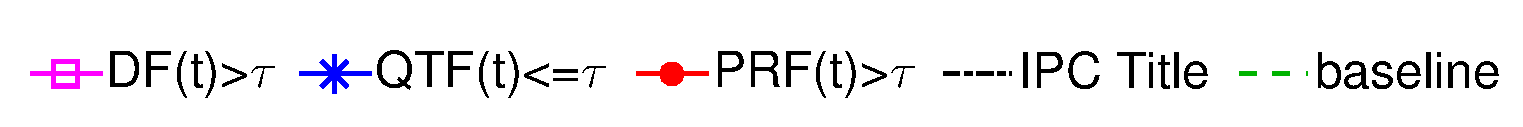
\includegraphics[width=9cm]{figs/l3}
\par\end{centering}

\begin{centering}
\subfigure[Mean Average Precision.]{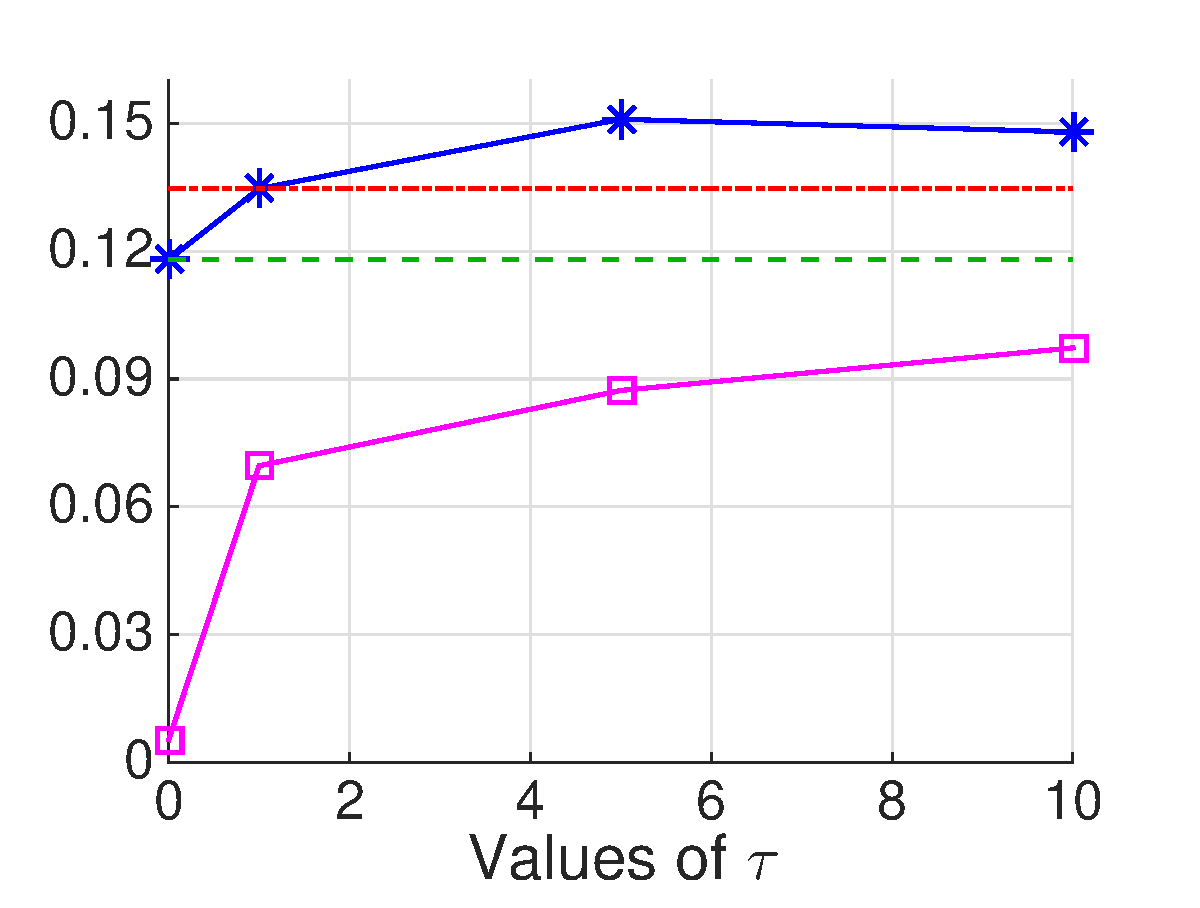
\includegraphics[width=6cm]{figs/fig3_map}} \hspace*{1.5cm} 
\subfigure[Average Recall.]{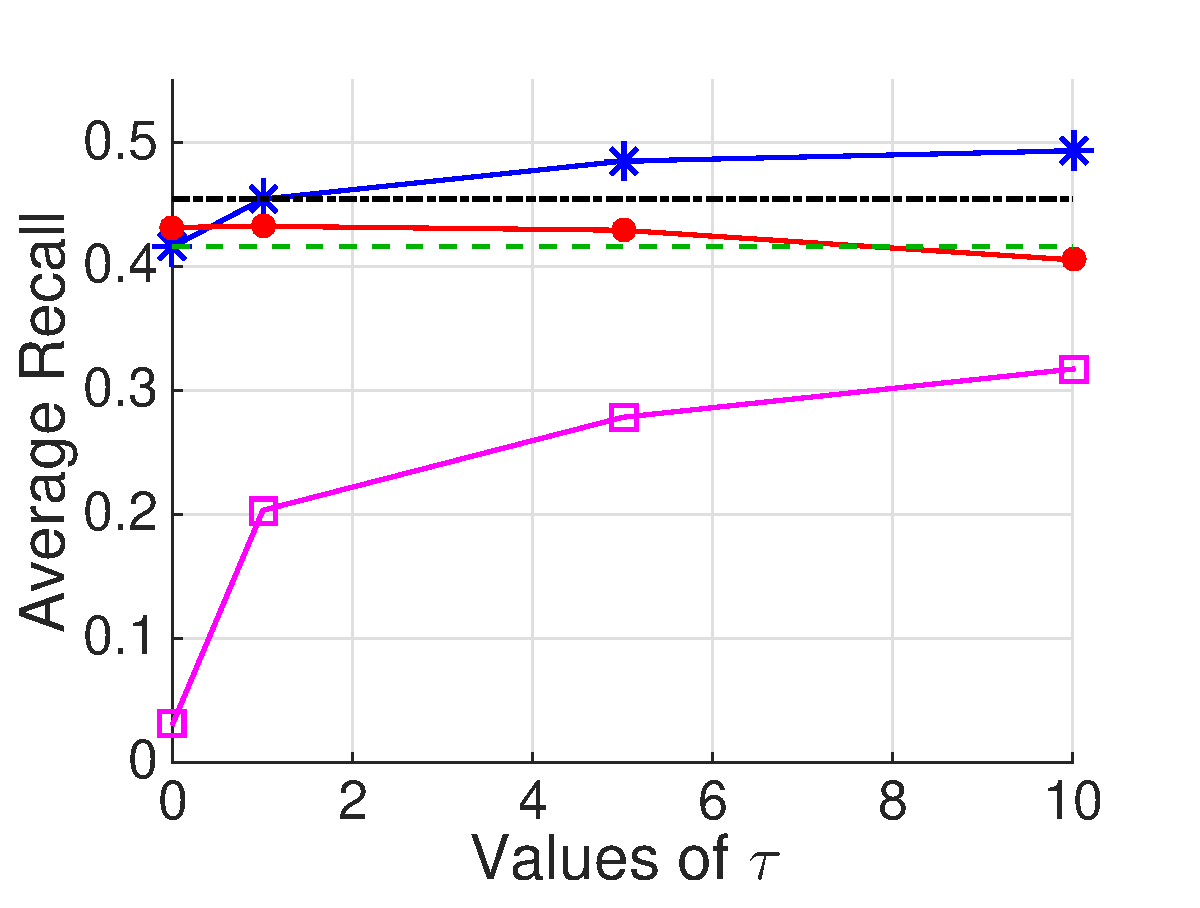
\includegraphics[width=6cm]{figs/fig3_recall}} 
\par\end{centering} 

\protect\caption{System performance versus the threshold $\tau$ for four different query reduction approaches.}
\label{fig:combinedapproach}
\end{figure}
%%%%%%%%%%%%%%%%%%%%%%%%%%%%%%%%%%%%%%%%%%%%%%%%%%%%%%%%%%%%%%
In standard IR, removing terms appearing highly frequently across documents in the collection can improve retrieval effectiveness~\citep{manning2008introduction}. Inspired by this fact, we hypothesise that we will improve the performance by pruning out highly frequent words in top-100 retrieved documents after an initial run of the patent query. To identify highly frequent terms, we calculate the average term frequency over top-100 documents for each term --- document frequent ($\mathit{DF}$) score --- as follows:
%%%%%%%%%%%%%%%%%%%%%%%%%%%%%%%%%%%%%%%%%%%%%%%%%%%%%%%%%%%%%%
\begin{equation}
 DF(t, Q)=\frac{1}{100}\sum_{d\in  D} TF(t, d),    
 \label{eq:df}
\end{equation}
where $D=\{d\in \mbox{Top-100 retrieved documents}\}$, and $TF(t, d)$ is the term frequency of each term in document $d$.
%\begin{displaymath}   t\in \lbrace \mbox{terms in top-100 retrieved documents}\rbrace\end{displaymath}
%%%%%%%%%%%%%%%%%%%%%%%%%%%%%%%%%%%%%%%%%%%%%%%%%%%%%%%%%%%%%%

We remove words with $\mathit{DF}$ score higher than $\tau$ ($DF(t, Q)>\tau$) from the patent query. 
As illustrated in Figure~\ref{fig:combinedapproach} (magenta line), such pruning hurts the performance. $\mathit{DF}$ pruning continues increasing and converges to the baseline as $\tau \to \infty $ (i.e., no pruning).
Overall, removing document frequent terms from patent query does not consider an appropriate approach since it ruins the performance. 
\subsubsection{Removing Infrequent Terms in Patent Query}
Frequent terms inside long and verbose queries are considered important~\cite{maxwell2013compact}. Thus, we hypothesize that removing terms appearing infrequently in the Patent Query may help and hence propose to remove terms with query term frequency (QTF) below a threshold $\tau$ ($QTF(t) \leq \tau$). Results in Figure~\ref{fig:combinedapproach} (blue line) indicate the performance is slightly better than the baseline when removing low QTF terms.  The best MAP is achieved when $\tau=5$ and it meets the baseline when $\tau=0$ (i.e., all terms retained). 
%In this approach the best value for the threshold is $\tau=5$ to get higher MAP.
\subsubsection{Removing Terms in IPC Titles}
The titles of IPC codes indicate the intended content of patents classified under that code by using a single phrase or several related phrases linked together. We used words in IPC code titles for each patent query as stopwords to reduce the query, based on the assumption that these terms are common to all patents having the same IPC code label.  As it can be seen in Figure~\ref{fig:combinedapproach} (black line), this approach slightly helps the performance.
\subsubsection{Query Reduction Using Pseudo Relevance Feedback}
% TODO: Must be consistent in either pruning or removing terms --- results should ideally converge to the baseline at 0.
% TODO: Should do simplest comparisons first and not combine pruning approaches.  Even better: evaluate methods mentioned in related work.
% TODO: What is an IPC title?  I don't know that this is... was it discussed?
Pseudo relevance feedback ($\mathit{PRF}$) is an automated process without user interaction which assumes the top \textit{k} ranked documents are relevant and the others are irrelevant~\citep{Baeza-Yates2011}. We use $\mathit{PRF}$ to select query terms~\cite{maxwell2013compact} --- the same as what we did for oracular relevance feedback system (Section~\ref{sec:oraculrquery}). We assume that top 5 retrieved documents are relevant and the rest are irrelevant, then we calculate $\mathit{PRF}$ score based on this assumption:  
%%%%%%%%%%%%%%%%%%%%%%%%%%%%%%%%%%%%%%%%%%%%%%%%%%%%%%%%%%%%%%
\begin{equation}
PRF(t,Q)=Rel(t)-Irr(t), 
 \label{eq:score}
\end{equation}
\vspace*{-2ex}
\begin{displaymath}t\in \lbrace \mbox{terms in top-100 retrieved documents}\rbrace,\end{displaymath}
%%%%%%%%%%%%%%%%%%%%%%%%%%%%%%%%%%%%%%%%%%%%%%%%%%%%%%%%%%%%%%  
where $\mathit{Rel(t)}$ is the average term frequency in top-5 retrieved patents, and $\mathit{Irr(t)}$ is
the average term frequency in the remained patents in top-100 retrieved documents.
We select the terms in the patent query that have the $\mathit{PRF}$ score higher than the threshold $\tau$ ($PRF(t)>\tau$) to reformulate a reduced query. Figure~\ref{fig:combinedapproach} (red line) shows that this approach is also unsuccessful at achieving a notable improvement over the baseline.
%%%%%%%%%%%%%%%%%%%%%%%%%%%%%%%%%%%%%%%%%%%%%%%%%%%%%%%%%%%%%%
%\begin{figure}[t!]
%   \centering
%   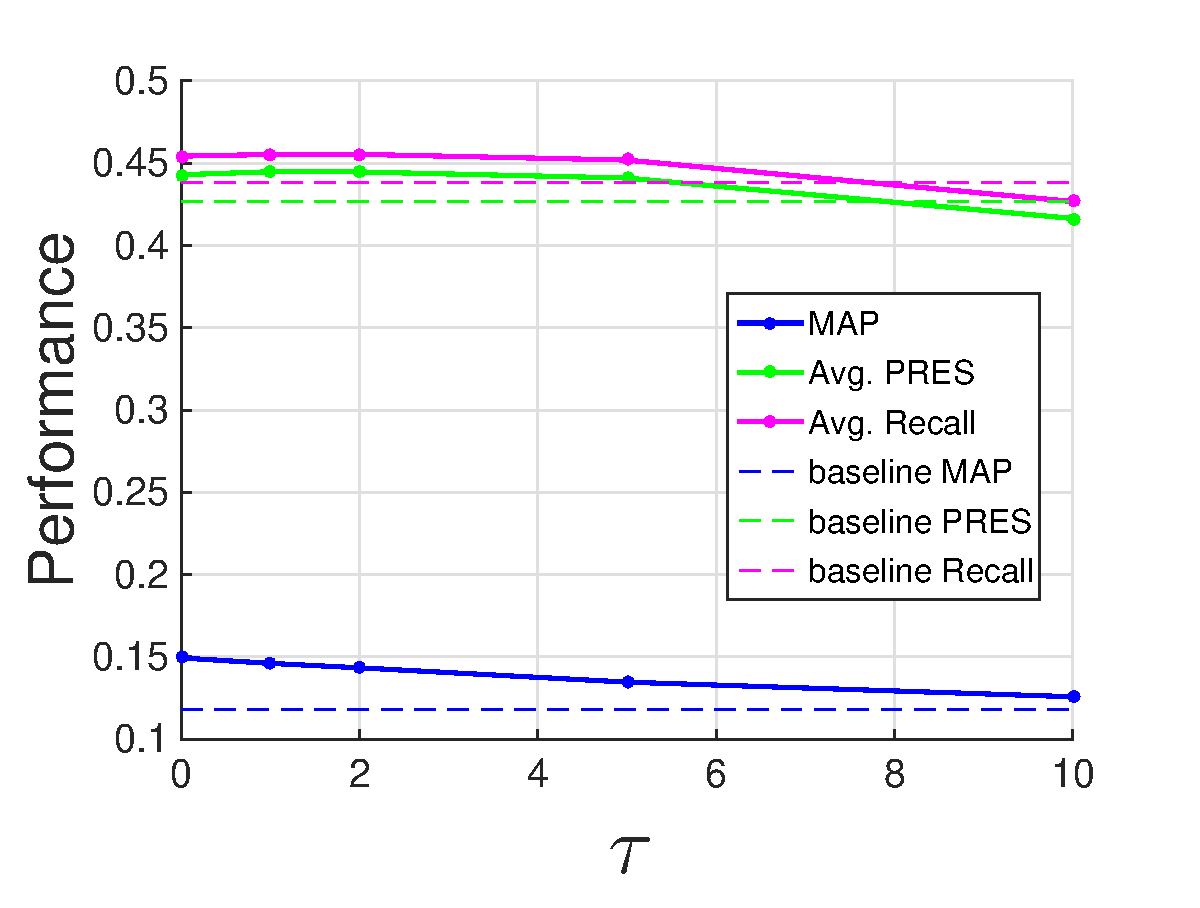
\includegraphics[width=0.50\textwidth,height=55mm]{figs/prf.eps}
%   \caption{Query reduction using PRF for various value of the threshold $\tau$.}   
%   \label{fig:prf} 
%\end{figure}
%%%%%%%%%%%%%%%%%%%%%%%%%%%%%%%%%%%%%%%%%%%%%%%%%%%%%%%%%%%%%%
\subsubsection{Automated Techniques Fails to Approximate Oracular Patent Query}
%%%%%%%%%%%%%%%%%%%%%%%%%%%%%%%%%%%%%%%%%%%%%%%%%%%%%%%%%%%%%%
%\begin{figure}[t!]
%\begin{centering}
%\subfigure[Query terms ($t \in Query$) versus Document Frequent terms.\label{fig:scatter_combined_a}]{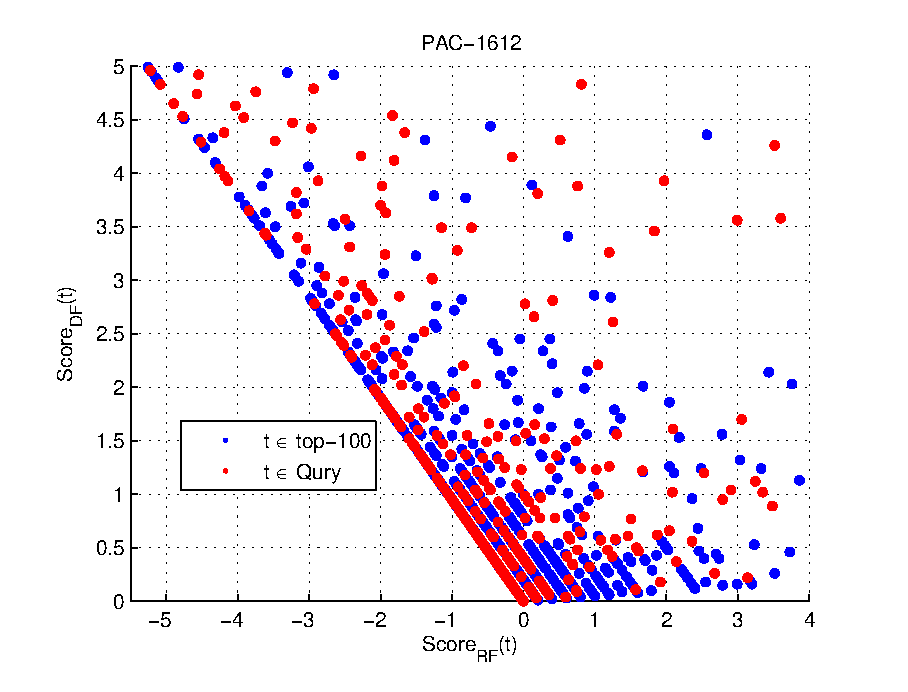
\includegraphics[width=9cm]{figs/qterm_rf_df.eps}} \hspace*{0.1cm}\\[1ex]% 
% %\subfigure[IPC Title words vs. Document Frequent terms.\label{fig:scatter_combined_b}]{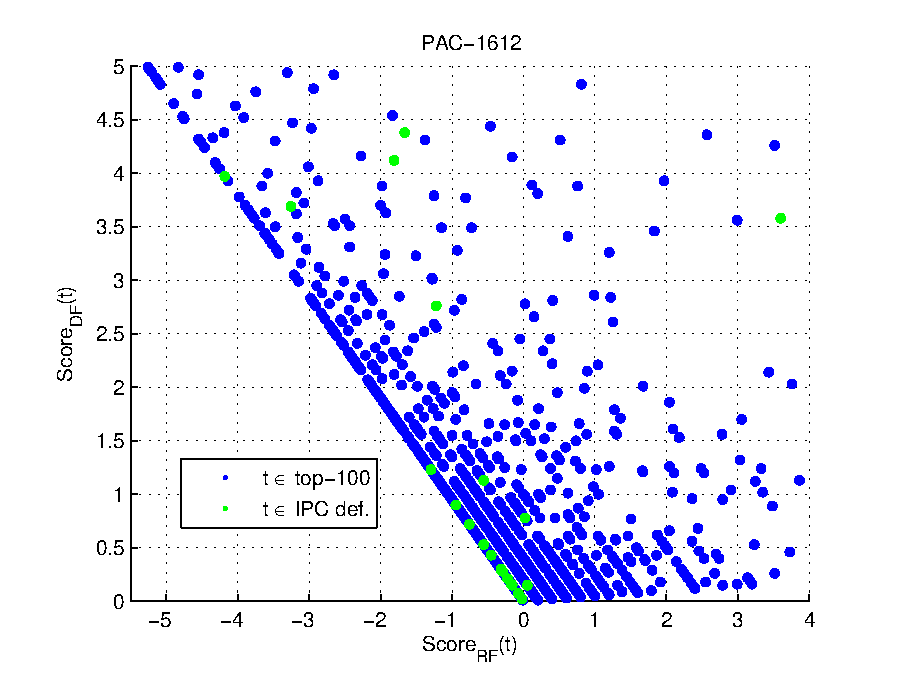
\includegraphics[width=7cm]{figs/ipcdef-rf-df.eps}} 
%\subfigure[Query terms ($t \in Query \; \bigwedge \; QTF(t)>5$) versus Document Frequent terms\label{fig:scatter_combined_b}]{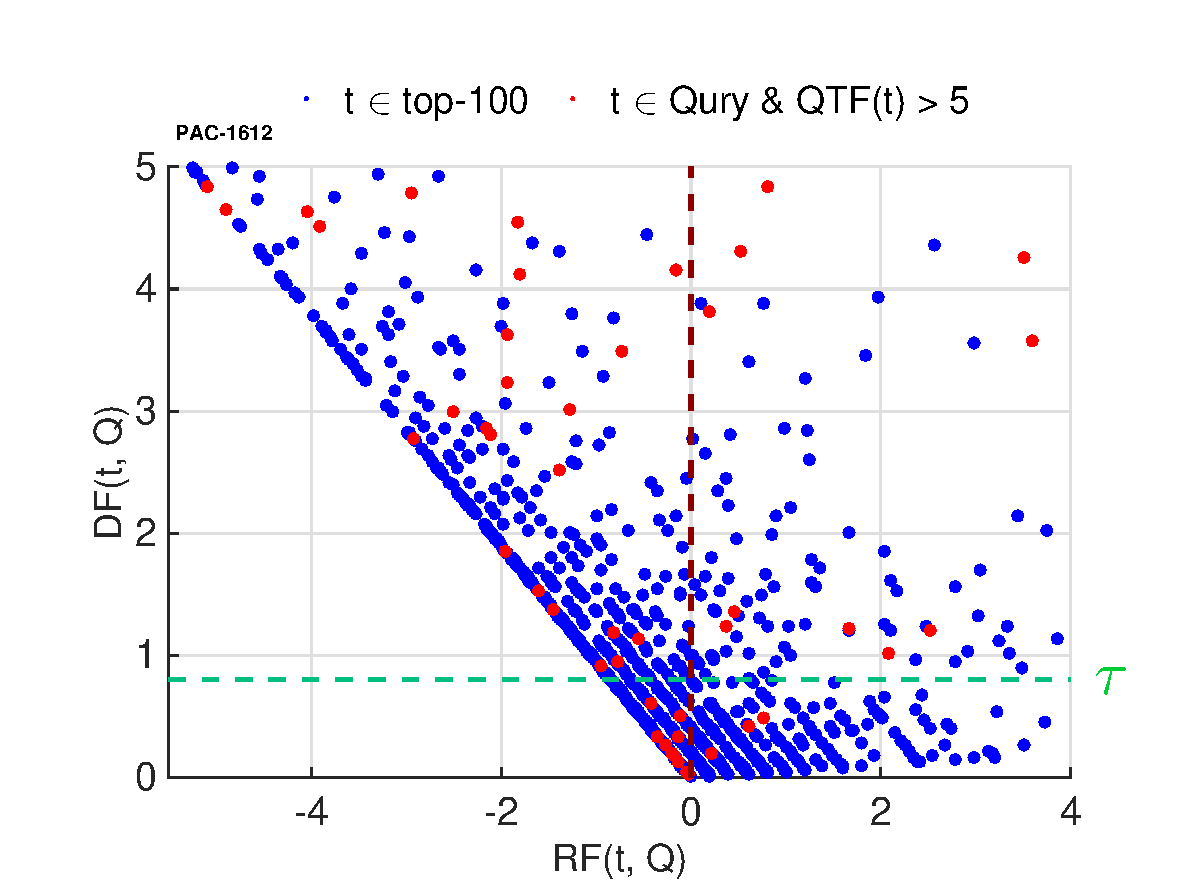
\includegraphics[width=9cm]{figs/df-rf-tauline.eps}}
%
%\par\end{centering}
%
%\protect\caption{Anecdotal example for simple query reduction approaches. Blue points are all terms in a vocabulary set made of top-100 retrieved documents and red points are terms in the patent query.}
%\label{fig:scatter_combined}
%\end{figure}
%%%%%%%%%%%%%%%%%%%%%%%%%%%%%%%%%%%%%%%%%%%%%%%%%%%%%%%%%%%%%%
In Section~\ref{sec:OracularQueryFormulation}, we showed that terms inside the patent query are sufficient to get a noticeable improvement over the baseline; 
however, results related to automated query reduction techniques showed only a little improvement. 
We analyse the causes through the following experiments.    

First, we use an anecdotal example --- a sample query --- to yse terms selected by proposed query reduction methods. 
Figure~\ref{fig:scatter_combined_a} shows a scatter plot of $\mathit{DF}$ score versus $\mathit{RF}$ score for the sample query --- PAC-1612. Each blue point is a vocabulary in top-100 retrieved document vocabulary set. We remark a negative correlation between $\mathit{DF(t, Q)}$ and $\mathit{RF(t, Q)}$ score; however it does not indicate that a term with a higher $\mathit{DF}$ score has essentially a lower $\mathit{RF}$ score.
Hence, if we prune it out in $\mathit{DF}$ pruning method, we are not essentially removing an unimportant term.
As it is illustrated in Figure~\ref{fig:scatter_combined_b}, by removing document frequent terms (e.g., $DF(t, Q)>\tau$), we also remove many useful terms (e.g., $RF(t, Q)>0$). In Figure~\ref{fig:scatter_combined_a}, red points are all query terms and in Figure~\ref{fig:scatter_combined_b}, they are query terms with term frequency higher than 5 (e.g., $QTF(t)>5$) --- where we got the best performance. 
Comparing Figures~\ref{fig:scatter_combined_a} and ~\ref{fig:scatter_combined_b} show that on the one hand, we are removing considerable amount of noisy terms by pruning out  terms with $QTF(t)<5$; on the other hand, we are also removing useful terms. In addition, remained terms are not purely useful terms because they are contaminated with the noisy terms. %We conclude that we achieve a trivial improvement over the baseline because proposed reduction techniques cannot precisely filter the noisy terms out. 
%%%%%%%%%%%%%%%%%%%%%%%%%%%%%%%%%%%%%%%%%%%%%%%%%%%%%%%%%%%%%%%%%%%%%%%%%%%%%%%%%%%%%%%%%%%%%%%%%%%%%%%%%%% 
%%%%%%%%%%%%%%%%%%%%%%%%%%%%%%%%%%%%%%%%%%%%%%%%%%%%%%%%%%%%%%
\begin{figure}[t!]
%\begin{centering}
%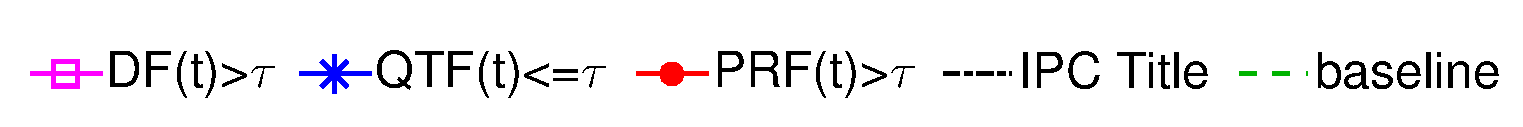
\includegraphics[width=9cm]{figs/l3}
%\par\end{centering}

\begin{centering}
\subfigure[Query terms ($t \in Query$) versus document frequent terms.\label{fig:scatter_combined_a}]{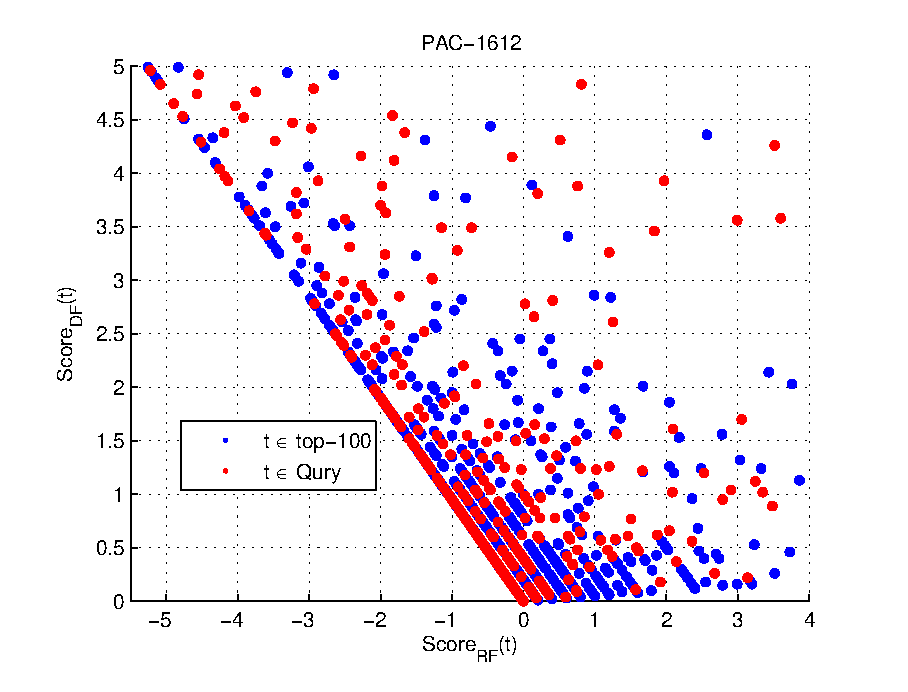
\includegraphics[width=7cm]{figs/qterm_rf_df.eps}} \hspace*{.1cm} 
\subfigure[Query terms ($t \in Query \; \bigwedge \; QTF(t)>5$) versus document frequent terms\label{fig:scatter_combined_b}]{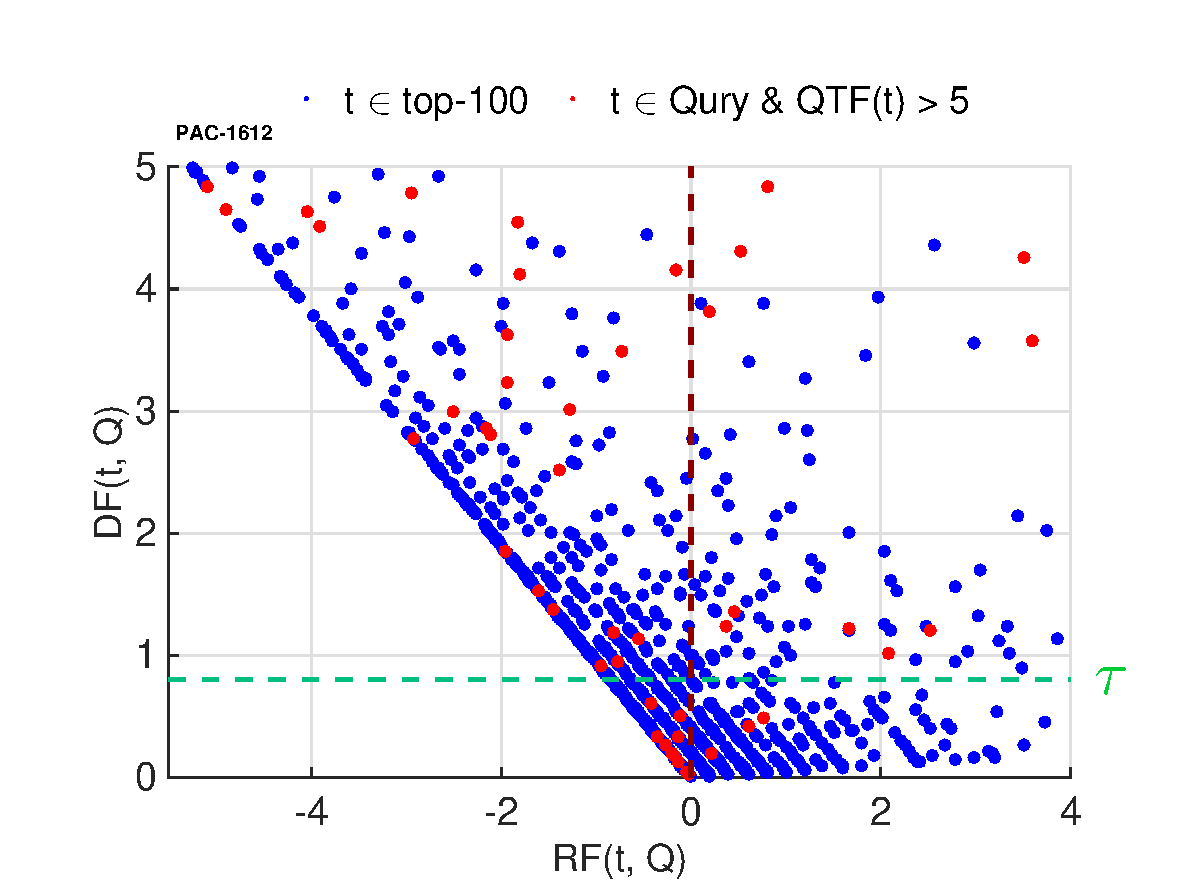
\includegraphics[width=7cm]{figs/df-rf-tauline.eps}} 
\par\end{centering} 

\protect\caption{Anecdotal example for simple query reduction approaches. Blue points are all terms in a vocabulary set made of top-100 retrieved documents and red points are terms in the patent query.}
\label{fig:scatter_combined}
\end{figure}
%%%%%%%%%%%%%%%%%%%%%%%%%%%%%%%%%%%%%%%%%%%%%%%%%%%%%%%%%%%%%%
%%%%%%%%%%%%%%%%%%%%%%%%%%%%%%%%%%%%%%%%%%%%%%%%%%%%%%%%%%%%%%
\begin{figure}[t!]
\begin{centering}
\subfigure[\label{fig:rf_prf_a}]{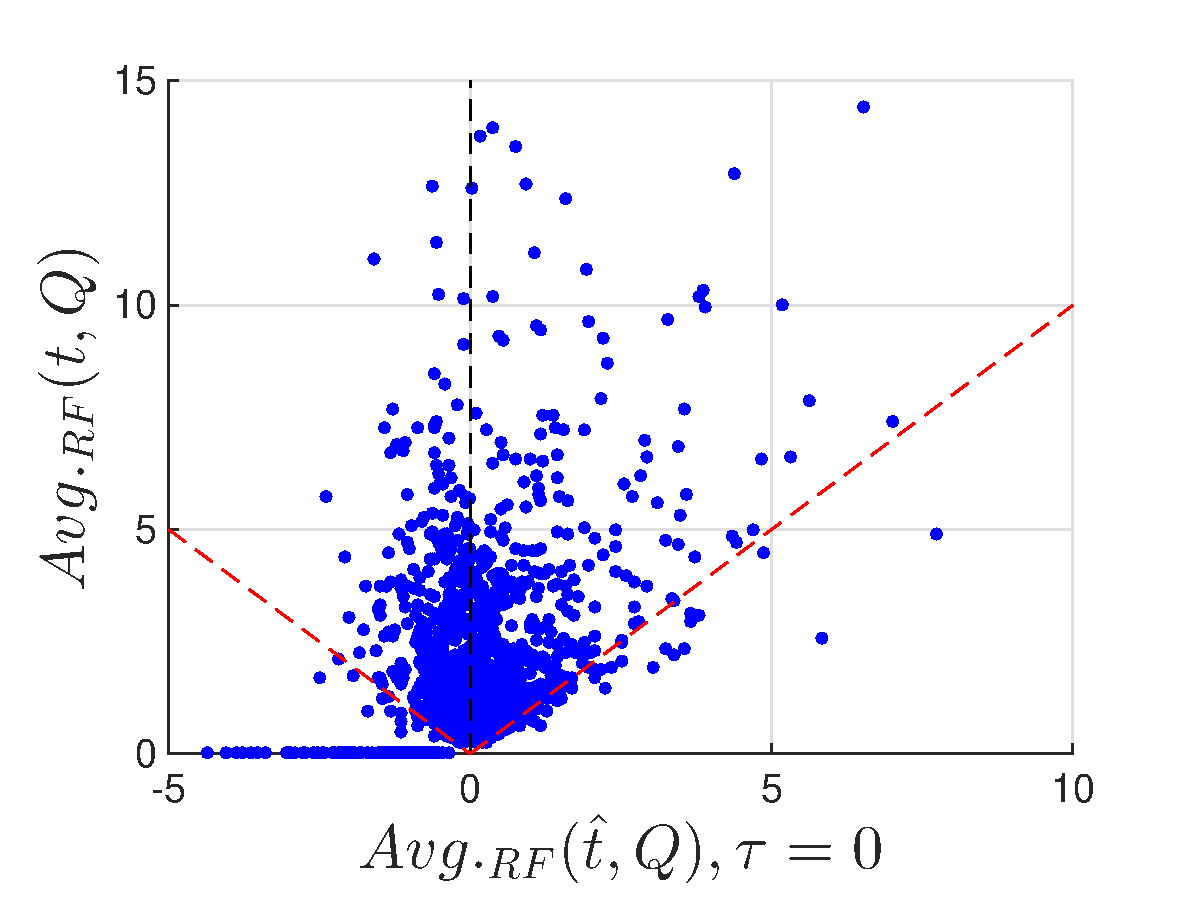
\includegraphics[width=7cm]{figs/scoretscorethat-tau0.eps}} \hspace*{0.1cm}
 \subfigure[\label{fig:rf_prf_b}]{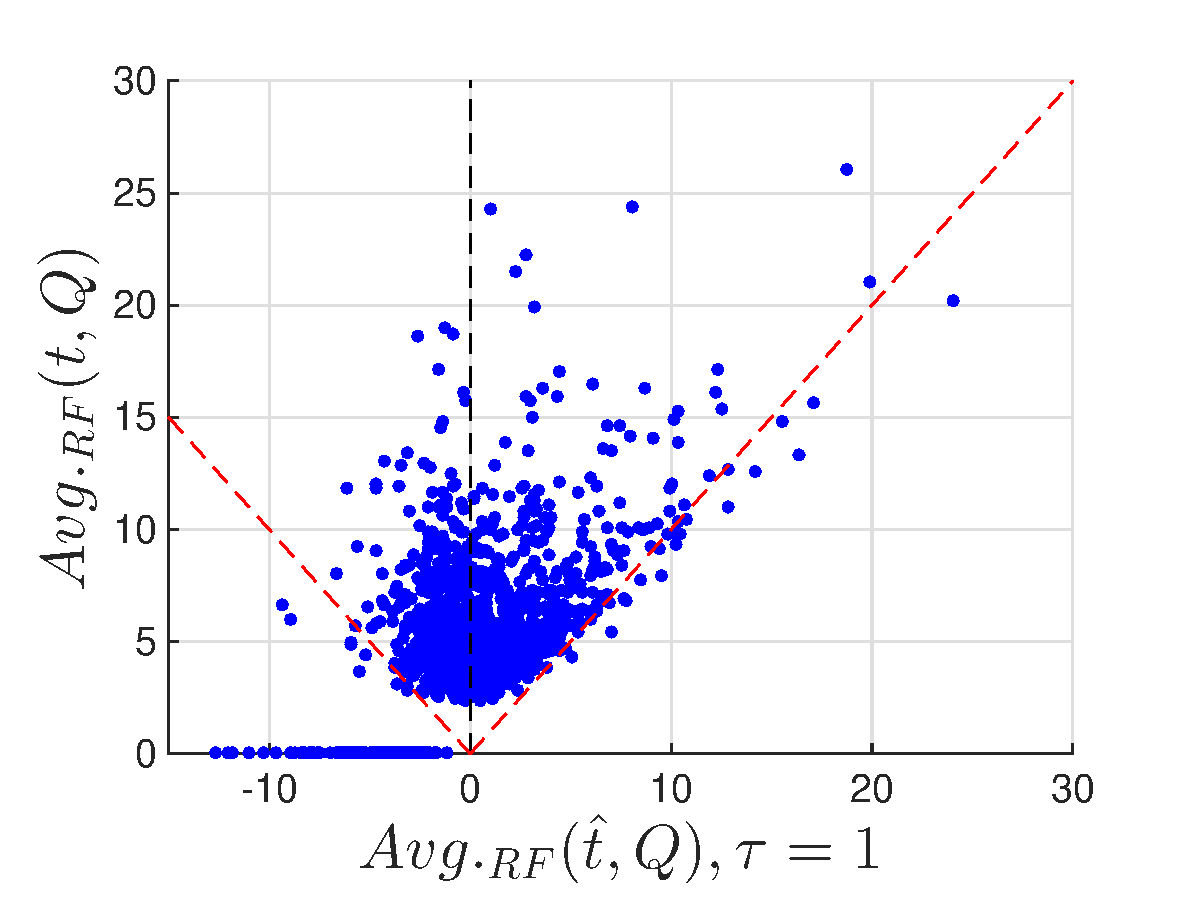
\includegraphics[width=7cm]{figs/scoretscorethat-tau1.eps}} \\[-1ex]% 
\subfigure[\label{fig:rf_prf_c}]{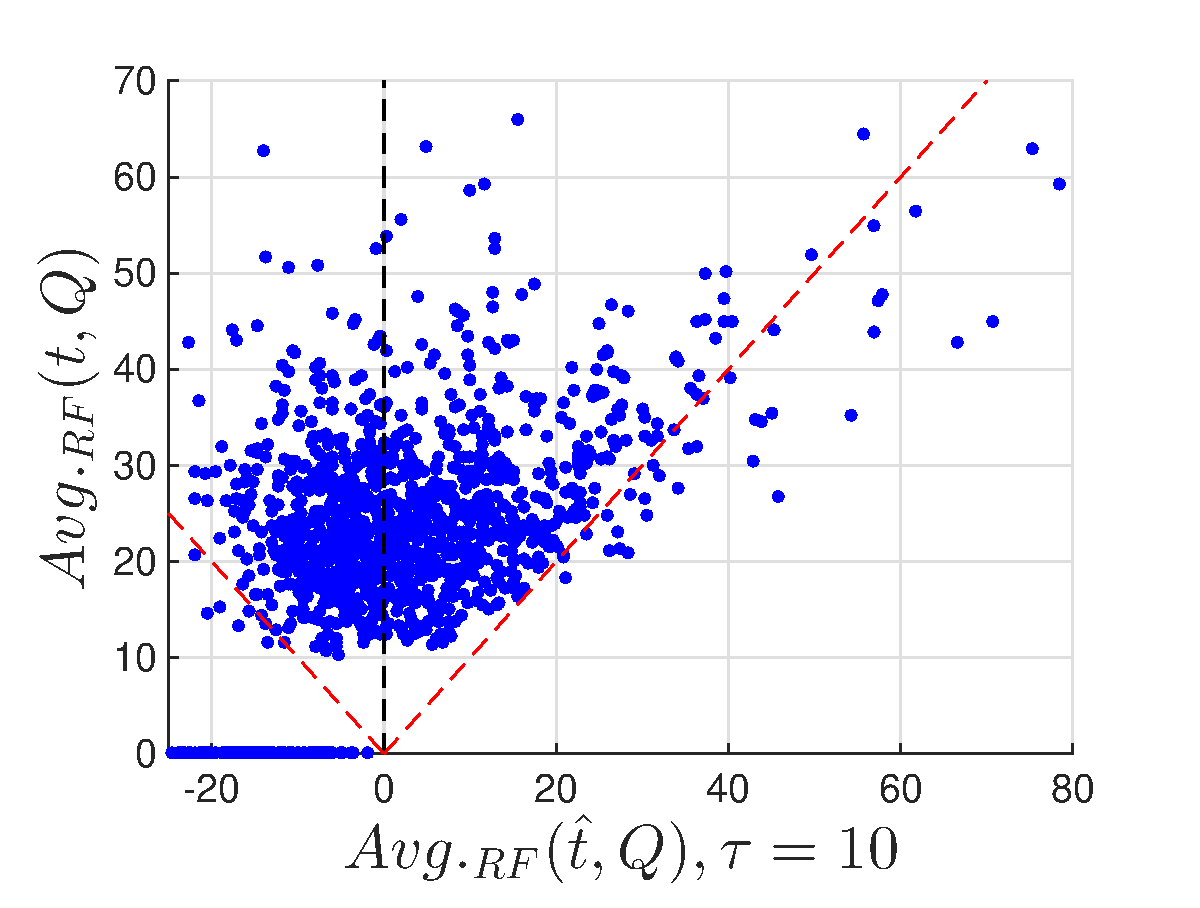
\includegraphics[width=7cm]{figs/scoretscorethat-tau10.eps}}

\par\end{centering}

\protect\caption{Comparing $\mathit{RF}$ score of top relevance feedback terms and top pseudo relevance feedback terms for three different values of the threshold $\tau$ (i.e., $0, 1, 10$).}
\label{fig:rf_prf}
\end{figure}
%%%%%%%%%%%%%%%%%%%%%%%%%%%%%%%%%%%%%%%%%%%%%%%%%%%%%%%%%%%%%%

In the second experiment, we analyse why the term selection technique using pseudo relevance feedback fails to approximate the oracular patent query.  
We seek for a pattern between top relevance feedback terms and top pseudo relevance feedback terms. For this purpose, we calculate the average $\mathit{RF}$ score of both terms with top  $\mathit{RF}$ score and terms with top $\mathit{PRF}$ score for each query as follows:
%%%%%%%%%%%%%%%%%%%%%%%%%%%%%%%%%%%%%%%%%%%%%%%%%%%%%%%%%%%%
\begin{equation}
Avg_{RF}(t, Q) = \frac{1}{|t|}\sum {RF}(t, Q), \;\;\;\; t\in \{t | RF(t, Q)>\tau\},
\end{equation}
%\begin{displaymath}t\in \{t | RF(t)>\tau\}\end{displaymath}
%%%%%%%%%%%%%%%%%%%%%%%%%%%%%%%%%%%%%%%%%%%%%%%%%%%%%%%%%%%%
\begin{equation}
Avg_{RF}(\hat{t}, Q) = \frac{1}{|\hat{t}|}\sum {RF}(\hat{t}, Q), \;\;\;\; \hat{t}\in \{\hat{t} | PRF(\hat{t}, Q)>\tau\},
\end{equation}
%\begin{displaymath}\hat{t}\in \{\hat{t} | PRF(\hat{t})>\tau\}\end{displaymath}
%%%%%%%%%%%%%%%%%%%%%%%%%%%%%%%%%%%%%%%%%%%%%%%%%%%%%%%%%%%%
where $Avg_{RF}(t, Q)$ is the average  $\mathit{RF}$ score for top  $\mathit{RF}$ terms ($RF(t, Q)>\tau$), $Avg_{RF}(\hat{t}, Q)$ is the average  $\mathit{RF}$ score for top  $\mathit{PRF}$ terms ($PRF(\hat{t}, Q)>\tau$), $\tau$ is a threshold for the score to select terms, $t$ is a symbol for terms with high $\mathit{RF}$ score and $\hat{t}$ is a symbol for terms with high $\mathit{PRF}$ score.

Figure~\ref{fig:rf_prf} shows a scatter plot of average $\mathit{RF}$ score for top relevance feedback terms and top pseudo relevance feedback terms. First, we observe that almost the $\mathit{RF}$ score of top relevance feedback terms is higher than the $\mathit{RF}$ score of top pseudo relevance feedback terms for almost all queries ($ Avg_{RF}(t, Q) > Avg_{RF}(\hat{t}, Q)$). We can also see that for about half of the queries, $Avg_{RF}(\hat{t}, Q)$ is negative that indicates we are selecting noisy terms by their pseudo relevance feedback score rather than useful terms. Second, we can find a very slight positive correlation toward selecting positive terms by pseudo relevance feedback, which is the reason that we could get a little improvement applying query reduction by $\mathit{PRF}$.  

Finally, we analyse the reasons that four proposed query reduction approaches fail to approximate the oracular patent query, using an anecdotal example of a sample query about an invention related to ``emulsifier''. 
Figure \ref{fig:anecdotal} shows the raw abstract of the invention, and the top high-scoring terms (except for IPC title terms which are not scored, but simply displayed) and their associated $\mathit{RF}$ scores for each approach. 
Terms are chosen based on the scores for each approach as follows: 
\begin{displaymath}\{t| DF(t)/QTF(t)/PRF(t)>10\}.\end{displaymath}
% Scott: the following is unclear... instead have modified Figure 3 caption.
%IPC title terms are the words appearing in the IPC title and do not have any score.
%\begin{displaymath}\{t| DF(t)/QTF(t)/PRF(t)>10\}\end{displaymath}
It can be seen that the four methods fail to clearly discriminate between useful and noisy terms.  Important stemmed terms like ``enzym'' and ``starch'' would be pruned according to $\mathit{DF}$; in contrast, $\mathit{QTF}$ and $\mathit{PRF}$ both score ``starch'' highly and retain it, but also retain other noisy terms.  Over half of the IPC title terms are noisy and appropriate to remove, but critical useful stemmed terms like ``emulsifi'' are also removed.
%As one example, important stemmed terms like ``enzym'' and ``starch'' have been removed by the DF pruning approach, which hurts query quality.  As another example, pruning IPC title terms removes highly noisy (negative) terms like ``amylos'' or ``saccharid'', but also removes useful terms like ``emulsifi''.  
%pruning IPC title terms yields more noisy terms than useful terms (13 out of 20 terms were noisy and removed, but more rare negative terms like ``amylos'' or ``saccharid'' remain).
  Critically, all methods retain noisy terms (red/negative) and results from Section~\ref{sec:OracularQueryFormulation} showed that the inclusion of even slightly noisy terms can significantly hurt performance.  Overall, all methods fail to retain only the oracular query terms (blue/positive) and do worse than PATATRAS.
%shows the raw abstract of the invention, and terms and their associated $\mathit{RF}$ scores for each approach. 
%Terms are chosen based on the scores for each approach as follows: 
%\begin{displaymath}\{t| DF(t)/QTF(t)/PRF(t)>10\}.\end{displaymath}
%%$\{t| DF(t)/QTF(t)/PRF(t)>10\}$.
%For the IPC title terms, all terms appearing in IPC title are displayed since they do not have any score.   
%It can be seen that the four methods fail clearly to discriminate between useful terms and noisy terms. As one example, important stemmed terms like ``enzym'' and ``starch'' have been removed by $\mathit{DF}$ pruning approach, which hurts the query quality.  As another example, retaining IPC code title terms yields more noisy terms than useful terms (19 out of 32, and few of them with a very negative score like ``amylos'' or ``saccharid''). This can justify slight improvement in performance when we prune terms in IPC title. Overall, all methods may retain highly negative terms and results from Section~\ref{sec:OracularQueryFormulation} showed that the inclusion of even slightly negative terms can significantly hurt the performance.
%In summary, we failed in approximating the Oracular Patent Query with any of four proposed Query reduction techniques.      
%%%%%%%%%%%%%%%%%%%%%%%%%%%%%%%%%%%%%%%%%%%%%%%%%%%%%%%%%%%%
\begin{figure}[htpb]
%\begin{figure}[t!]
\begin{framed}
\vspace*{-2ex}
  \centering
    %\lstinputlisting[frame=single, basicstyle=\scriptsize\ttfamily , linewidth=\columnwidth,breaklines=true]{code/anecdotale.tex}\vspace*{-2ex}
 \begin{lstlisting}[basicstyle=\small\ttfamily , linewidth=\columnwidth,breaklines=true, language=TeX] 
PAC-1293

Abstract: The invention relates to an emulsifier, a method for 
preparing said emulsifier, and to its use in various applications
, primarily food and cosmetic applications. The invention also 
relates to the use of said emulsifier for the creation of an 
elastic, gelled foam. An emulsifier according to the invention is 
based on a starch which is enzymatically converted, using a 
specific type of enzyme, and modified in a specific 
esterification reaction.

(1) DF Terms: <@\textcolor{blue}{starch:14.64}@>, <@\textcolor{blue}{enzym:29.49}@>, <@\textcolor{red}{amylos:-20.15}@>, 
<@\textcolor{blue}{oil:8.63}@>, <@\textcolor{red}{dispers:-8.66}@>, <@\textcolor{red}{ph:-4.55}@>, <@\textcolor{red}{dry:-6.21}@>, <@\textcolor{red}{heat:-2.26}@>, 
<@\textcolor{red}{product:-5.48}@>, <@\textcolor{red}{slurri:-11.48}@>, <@\textcolor{blue}{viscos:7.77}@>, <@\textcolor{red}{composit:-4.49}@>, 
<@\textcolor{red}{reaction:-1.97}@>, <@\textcolor{red}{food:-11.94}@>, <@\textcolor{blue}{agent:5.19}@>, <@\textcolor{red}{debranch:-10.58}@>, 
<@\textcolor{red}{reduc:-6.37}@>, <@\textcolor{red}{fat:-12.83}@>, <@\textcolor{red}{prepar:-0.82}@>, <@\textcolor{red}{hour:-5.42}@>, 
<@\textcolor{blue}{waxi:19.41}@>, <@\textcolor{blue}{deriv:11.97}@>, <@\textcolor{red}{content:-3.38}@>, <@\textcolor{blue}{aqueou:0.38}@>, 
<@\textcolor{red}{saccharid:-11.95}@>, <@\textcolor{red}{ml:-0.79}@>, <@\textcolor{red}{cook:-10.04}@>, <@\textcolor{blue}{modifi:5.65}@>, 
<@\textcolor{blue}{solid:5.50}@>, <@\textcolor{blue}{sampl:6.27}@>, <@\textcolor{blue}{mix:2.48}@>, <@\textcolor{red}{minut:-1.68}@>, <@\textcolor{red}{dri:-0.91}@>, 
<@\textcolor{red}{gel:-9.85}@>, <@\textcolor{blue}{activ:5.98}@>, <@\textcolor{red}{corn:-5.27}@>, <@\textcolor{blue}{alpha:12}@>, <@\textcolor{red}{sprai:-2.74}@> 

(2) QTF Terms: <@\textcolor{blue}{starch:14.64}@>, <@\textcolor{blue}{emulsifi:6.72}@>, <@\textcolor{red}{succin:-3.46}@>, 
<@\textcolor{blue}{enzym:29.49}@>, <@\textcolor{blue}{emuls:12.66}@>, <@\textcolor{blue}{hydrophob:5.45}@>, <@\textcolor{red}{anhydrid:-5.47}@>, 
<@\textcolor{red}{reaction:-1.97}@>, <@\textcolor{red}{octenyl:-0.66}@>, <@\textcolor{blue}{stabil:3.64}@>, <@\textcolor{blue}{alkenyl:0.06}@>, 
<@\textcolor{blue}{reagent:1.17}@>, <@\textcolor{blue}{carbon:0.12}@>, <@\textcolor{blue}{potato:3.74}@>, <@\textcolor{red}{alkyl:-0.33}@>, 
<@\textcolor{red}{wt:-4.57}@>, <@\textcolor{blue}{ether:1.96}@>, <@\textcolor{red}{enzymat:-3.45}@>, <@\textcolor{blue}{convers:10.44}@>, 
<@\textcolor{red}{chain:-5.53}@>, <@\textcolor{blue}{atom:0.03}@>, <@\textcolor{red}{ph:-4.55}@>, <@\textcolor{red}{treat:-0.89}@>, 
<@\textcolor{red}{ammonium:-1.96}@>, <@\textcolor{red}{food:-11.94}@>, <@\textcolor{red}{amylos:-20.15}@>, 
<@\textcolor{red}{glucanotransferas:-0.86}@>, <@\textcolor{red}{glycidyl:-0.40}@>, <@\textcolor{red}{glycosyl:-0.02}@>, 
<@\textcolor{red}{dry:-6.21}@>, <@\textcolor{blue}{deriv:11.97}@>, <@\textcolor{blue}{transferas:0.89}@>, <@\textcolor{red}{foam:-0.49}@>, 

(3) IPC title Terms:<@\textcolor{blue}{cosmet:3.77}@>, <@\textcolor{blue}{toilet:0.18}@>, <@\textcolor{red}{prepar:-0.82}@>, 
<@\textcolor{blue}{case:0.47}@>, <@\textcolor{red}{accessori:-0.01}@>, <@\textcolor{red}{store:-0.37}@>, <@\textcolor{blue}{handl:0.07}@>, 
<@\textcolor{red}{pasti:-0.17}@>, <@\textcolor{red}{substanc:-1.21}@>, <@\textcolor{red}{fibrou:-0.01}@>, <@\textcolor{red}{pulp:-1.28}@>, 
<@\textcolor{red}{constitut:-0.06}@>, <@\textcolor{blue}{paper:1.26}@>, <@\textcolor{red}{impregn:-0.11}@>, <@\textcolor{blue}{emulsifi:6.72}@>, 
<@\textcolor{red}{wet:-0.28}@>, <@\textcolor{red}{dispers:-8.66}@>, <@\textcolor{red}{foam:-0.49}@>, <@\textcolor{red}{produc:-0.57}@>, 
<@\textcolor{blue}{agent:5.19}@>, <@\textcolor{blue}{relev:0.18}@>, <@\textcolor{blue}{class:0.053}@>, <@\textcolor{red}{lubric:-0.38}@>, 
<@\textcolor{blue}{emuls:12.66}@>, <@\textcolor{red}{fuel:-0.011}@>, <@\textcolor{blue}{deriv:11.97}@>, <@\textcolor{blue}{starch:14.64}@>, 
<@\textcolor{red}{amylos:-20.15}@>, <@\textcolor{red}{compound:-0.63}@>, <@\textcolor{red}{saccharid:-11.95}@>, 
<@\textcolor{blue}{radic:1.03}@>, <@\textcolor{red}{acid:-3.19}@> 

(4) PRF Terms: <@\textcolor{blue}{starch:14.64}@>, <@\textcolor{blue}{encapsul:17.50}@>, <@\textcolor{red}{chees:-4.22}@>, 
<@\textcolor{blue}{oil:8.63}@>, <@\textcolor{blue}{hydrophob:5.45}@>, <@\textcolor{blue}{agent:5.19}@>, <@\textcolor{red}{casein:-2.19}@>, 
<@\textcolor{blue}{degrad:17.13}@>, <@\textcolor{blue}{deriv:11.97}@>, <@\textcolor{blue}{tablet:5.30}@>, <@\textcolor{red}{debranch:-10.58}@>, 
<@\textcolor{red}{imit:-1.13}@>, <@\textcolor{blue}{viscos:7.77}@>, <@\textcolor{blue}{oxid:5.97}@>, <@\textcolor{blue}{activ:5.98}@>, <@\textcolor{blue}{osa:9.32}@>, 
<@\textcolor{blue}{funnel:2.68}@>, <@\textcolor{blue}{amylas:26.06}@>, <@\textcolor{red}{amylopectin:-7.14}@>, <@\textcolor{blue}{maiz:20.61}@>, 
<@\textcolor{red}{blend:-3.17}@>, <@\textcolor{blue}{waxi:19.41}@>, <@\textcolor{blue}{convert:31.81}@>, 

 \end{lstlisting} 
 \vspace*{-2ex}
\end{framed}
 \vspace*{-2ex}
  \caption{The top terms scored by each of four methods on a sample
    query (except for IPC title terms which are not scored); whether the term is
    pruned or retained depends on each approach.
    Numerical oracular scores $\mathit{RF}(t,Q)$ are provided
    indicating whether the term was actually useful (blue/positive) or
    noisy (red/negative).}
  \label{fig:anecdotal}  
\end{figure}
\FloatBarrier
%%%%%%%%%%%%%%%%%%%%%%%%%%%%%%%%%%%%%%%%%%%%%%%%%%%%%%%%%%%%
%\newpage
\subsection{Semi-automated Interactive Reduction}
\label{sec:SemiAutomatedInteractiveReduction}
Our sample analysis of specific queries and terms selected via our oracular
approach suggests that automated methods fall far short of optimal term selection.
This leads us to explore another approach of approximating the oracular query
derived from relevance judgements by using a subset of relevance judgements
through interactive methods. Specifically, to minimize the need for user interaction,
in this section we analyse the performance of an oracular query derived from
only the first relevant document identified in the search results.
%\begin{comment}
%All our attempts to improve the system effectiveness without accessing the relevance feedback were quite in vein because the features we recognized were tightly the combination of the useful words and noisy words and the system performance is too sensitive to the existence of a noisy word or the absence of the useful terms. So, we decided to apply much more realistic approach in which feedback terms are extracted only from the first ranked relevant document retrieved. 
%\end{comment}
Using this approach, Table \ref{tab:firstrel} shows that we can double the MAP in comparison to our baseline and also outperform the PATATRAS system.

Furthermore, to establish the minimal interaction required by this
approach, Figure \ref{fig:FirstTPRankHisto} indicates that the
baseline methods return a relevant patent approximately 80\% of the
time in the first 10 results and 90\% of the time in the first 20
results.  Hence, such an interactive approach requires relatively low
user effort while achieving state-of-the-art performance.
%%%%%%%%%%%%%%%%%%%%%%%%%%%%%%%%%%%%%%%%%%%%%%%%%%%%%%%%%%%%%%%%
\begin{table}[t!]
  \begin{center}
   \caption{System performance using minimal relevance feedback. $\tau$ is $\mathit{RF}$ score threshold, and $k$ indicates the number of first relevant retrieved patents.}\vspace{3mm}
  \input table/partialRFtermselect.tex   
  \label{tab:firstrel}
  \end{center}  
\end{table}
%\FloatBarrier
%%%%%%%%%%%%%%%%%%%%%%%%%%%%%%%%%%%%%%%%%%%%%%%%%%%%%%%%%%%%%%%%
%%%%%%%%%%%%%%%%%%%%%%%%%%%%%%%%%%%%%%%%%%%%%%%%%%%%%%%%%%%%%%%%
\begin{figure}[t!]
\begin{centering}
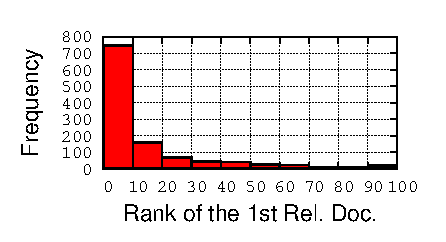
\includegraphics[width=6.5cm, height=3.5cm]{figs/1stRank}
\par\end{centering}

\protect\caption{The distribution of the first relevant document rank over test queries.}
\label{fig:FirstTPRankHisto}
\end{figure}
%\FloatBarrier
%%%%%%%%%%%%%%%%%%%%%%%%%%%%%%%%%%%%%%%%%%%%%%%%%%%%%%%%%%%%%%%%
%%%%%%%%%%%%%%%%%%%%%%%%%%%%%%%%%%%%%%%%%%%%%%%%%%%%%%%%%%%%%%%%
%%%%%%%%%%%%%%%%%%%%%%%%% SECTION 4 %%%%%%%%%%%%%%%%%%%%%%%%%%
%%%%%%%%%%%%%%%%%%%%%%%%%%%%%%%%%%%%%%%%%%%%%%%%%%%%%%%%%%%%%%
%\section{Summary}

